\documentclass[11pt,aspectratio=169]{beamer}

\usetheme{Madrid}
\usecolortheme{default}
\setbeamertemplate{navigation symbols}{}
\setbeamertemplate{footline}[frame number]

\usepackage{amsmath,amssymb}
\usepackage{graphicx}
\usepackage{booktabs}
\usepackage{tikz}
\usetikzlibrary{arrows.meta,positioning,fit,backgrounds,shapes.geometric,calc,decorations.pathreplacing,decorations.pathmorphing,patterns}

% Notation shortcuts
\newcommand{\Treq}{T^{\text{req}}}
\newcommand{\Tacq}{T^{\text{acq}}}
\newcommand{\Tarr}{T^{\text{arr}}}
\newcommand{\Trel}{T^{\text{rel}}}

\title{Discrete Event Traffic Simulation Framework\\using Object-Driven Cellular Automata}
\subtitle{Ongoing work from PhD dissertation --- to be submitted to\\Transportation Research Part B: Methodological}
\author{Kerem Demirtas \and Pitu Mirchandani \and Xuesong Zhou}
\institute[ASU]{%
  Kerem Demirtas, Pitu Mirchandani\\
  School of Computing and Augmented Intelligence\\
  Arizona State University
  \and
  Xuesong Zhou\\
  School of Sustainable Engineering and the Built Environment\\
  Arizona State University}
\date{}

\begin{document}

% ----------------------------------------------------------
\begin{frame}
\titlepage
\end{frame}

% ----------------------------------------------------------
\begin{frame}{Outline}
\tableofcontents
\end{frame}

% ==========================================================
\section{Motivation}
% ==========================================================

% ----------------------------------------------------------
\begin{frame}{Traffic Simulation: Two Dominant Paradigms}
\begin{columns}[T]
% --- Left column: Microscopic Simulators ---
\begin{column}{0.48\textwidth}
\begin{center}
{\small\bfseries Microscopic Simulators}\\[1pt]
{\scriptsize SUMO, Vissim, CORSIM}\\[3pt]
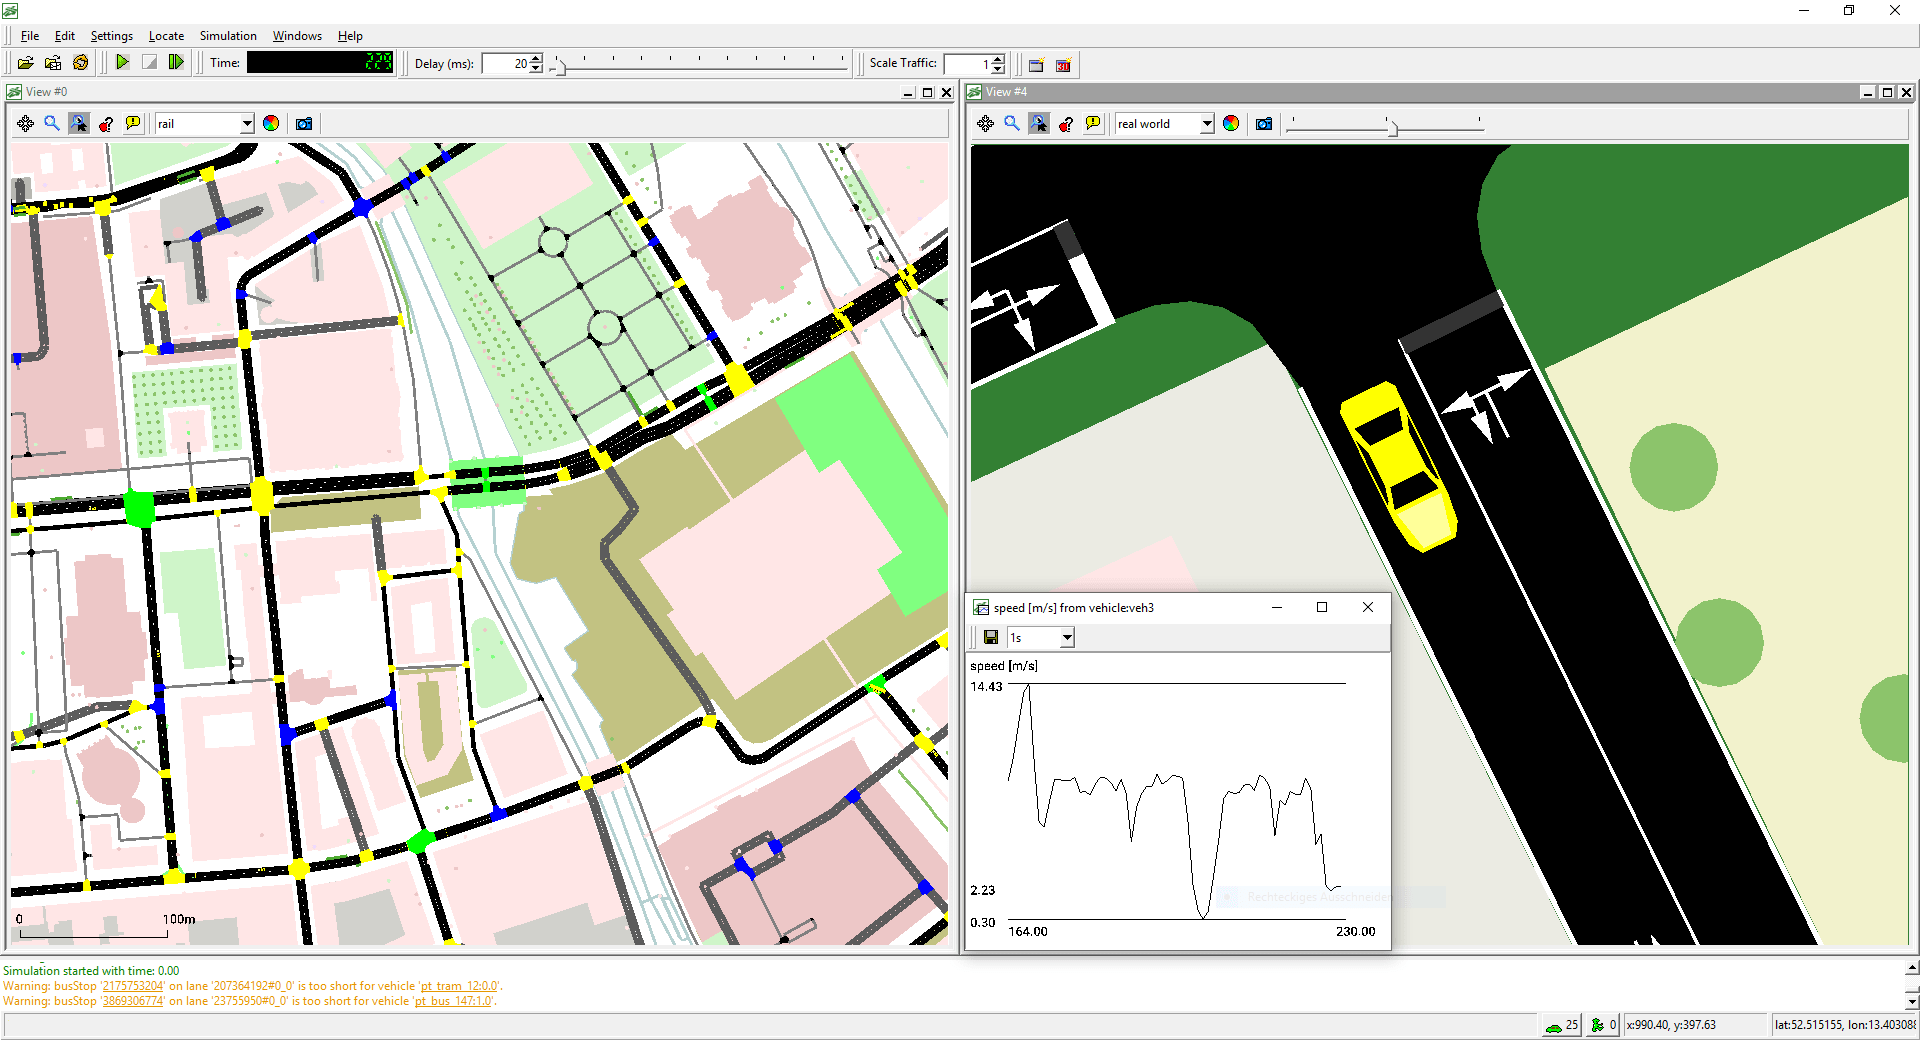
\includegraphics[width=\linewidth,height=3cm,keepaspectratio]{sumo_screenshot.png}
\end{center}
\vspace{3pt}
{\scriptsize\color{green!50!black}
+ Individual vehicles\\
+ High-fidelity CF/LC}\\[2pt]
{\scriptsize\color{red!70!black}
-- Fixed timestep $\Delta t$\\
-- Every vehicle, every step\\
-- Cost: $O(N \times T / \Delta t)$}
\end{column}
% --- Right column: Cellular Automata ---
\begin{column}{0.48\textwidth}
\begin{center}
{\small\bfseries Cellular Automata}\\[1pt]
{\scriptsize NaSch {\tiny[3]}, Rickert {\tiny[4]}, Knospe {\tiny[5]}}\\[3pt]
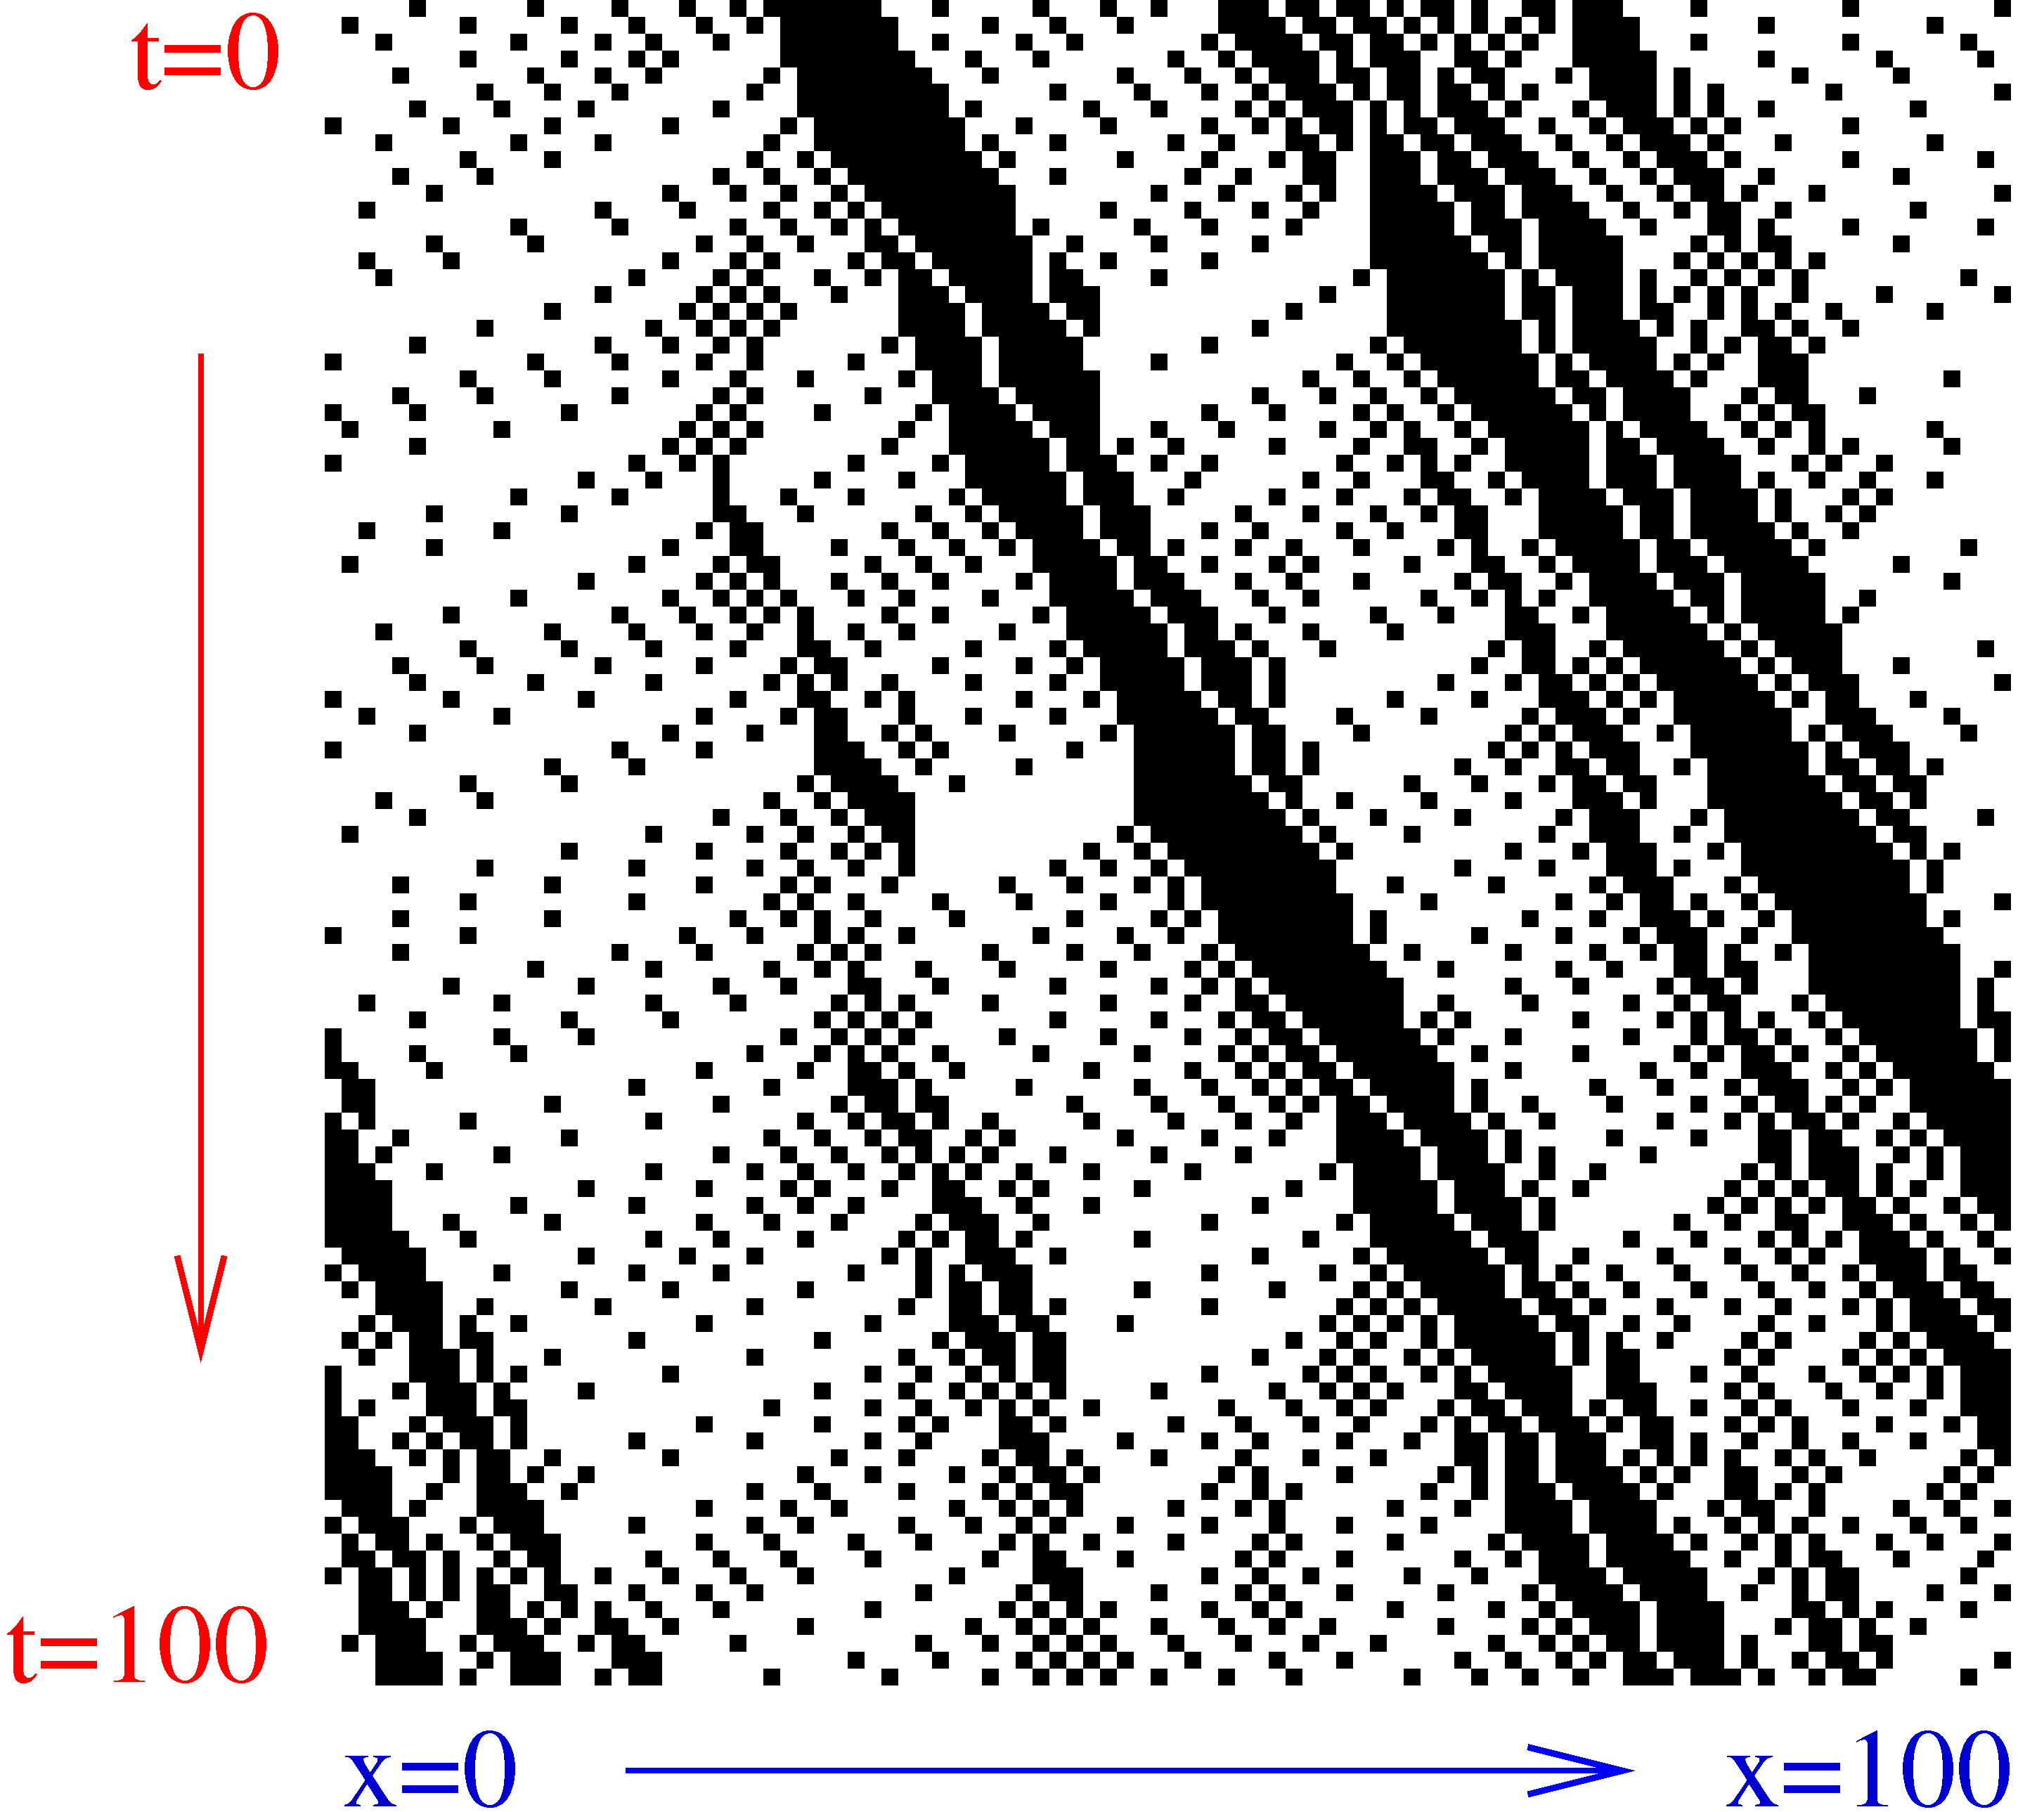
\includegraphics[width=\linewidth,height=3cm,keepaspectratio]{nasch_screenshot.png}
\end{center}
\vspace{3pt}
{\scriptsize\color{green!50!black}
+ Simple rules, fast\\
+ Discrete cells}\\[2pt]
{\scriptsize\color{red!70!black}
-- Synchronous updates\\
-- Integer speeds only\\
-- Stepped FD artifacts}
\end{column}
\end{columns}

\vfill
\begin{center}
\fcolorbox{red!50}{red!10}{\parbox{0.85\textwidth}{\centering\small
\alert{Shared limitation:} time advances in fixed increments --- global clock synchronization}}
\end{center}
\end{frame}

% ----------------------------------------------------------
\begin{frame}{Why Is Fixed-Timestep a Problem?}
\begin{center}
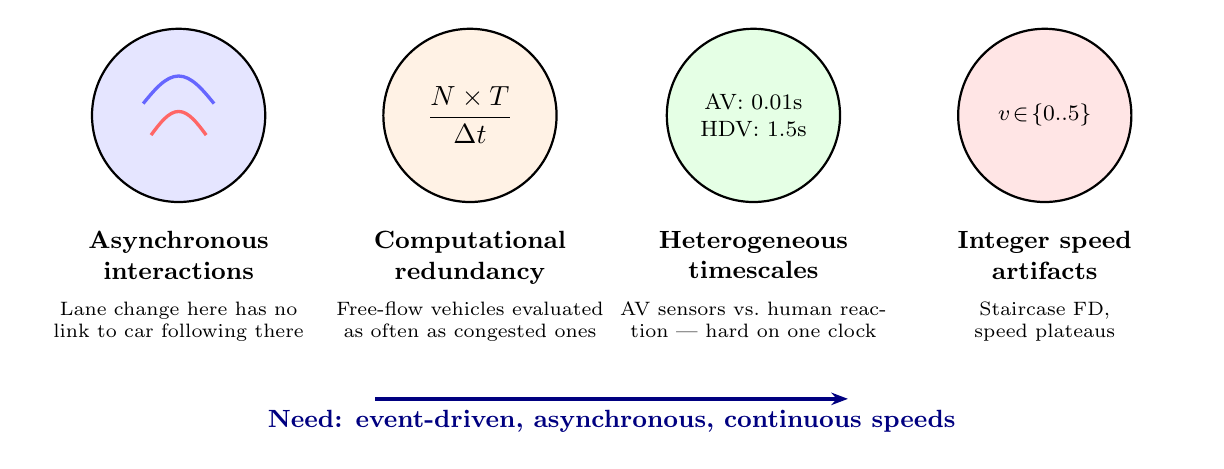
\begin{tikzpicture}[
    icon/.style={draw, circle, minimum size=2.2cm, thick, inner sep=2pt, align=center},
    lbl/.style={font=\small\bfseries, anchor=north, text width=3.2cm, align=center},
    desc/.style={font=\scriptsize, anchor=north, text width=3.6cm, align=center},
]
% Four visual concepts in a row
% 1. Asynchronous
\node[icon, fill=blue!10] (a1) at (-5.5,0) {};
\draw[very thick, blue!60] (-5.95,0.15) sin (-5.5,0.5) cos (-5.05,0.15);
\draw[very thick, red!60] (-5.85,-0.25) sin (-5.5,0.05) cos (-5.15,-0.25);
\node[lbl] at (-5.5,-1.35) {Asynchronous\\interactions};
\node[desc] at (-5.5,-2.25) {Lane change here has no link to car following there};

% 2. Redundancy
\node[icon, fill=orange!10, font=\normalsize] (a2) at (-1.8,0) {$\dfrac{N \times T}{\Delta t}$};
\node[lbl] at (-1.8,-1.35) {Computational\\redundancy};
\node[desc] at (-1.8,-2.25) {Free-flow vehicles evaluated as often as congested ones};

% 3. Heterogeneous timescales
\node[icon, fill=green!10, font=\footnotesize] (a3) at (1.8,0) {AV: 0.01s\\HDV: 1.5s};
\node[lbl] at (1.8,-1.35) {Heterogeneous\\timescales};
\node[desc] at (1.8,-2.25) {AV sensors vs.\ human reaction --- hard on one clock};

% 4. Integer speed
\node[icon, fill=red!10, font=\footnotesize] (a4) at (5.5,0) {$v\!\in\!\{0..5\}$};
\node[lbl] at (5.5,-1.35) {Integer speed\\artifacts};
\node[desc] at (5.5,-2.25) {Staircase FD,\\speed plateaus};

% Bottom arrow
\draw[-{Stealth[length=6pt]}, very thick, blue!50!black] (-3,-3.6) -- (3,-3.6)
    node[midway, below, font=\small\bfseries] {Need: event-driven, asynchronous, continuous speeds};
\end{tikzpicture}
\end{center}
\end{frame}

% ----------------------------------------------------------
\begin{frame}{Our Proposal: ODCA-DES}
\begin{center}
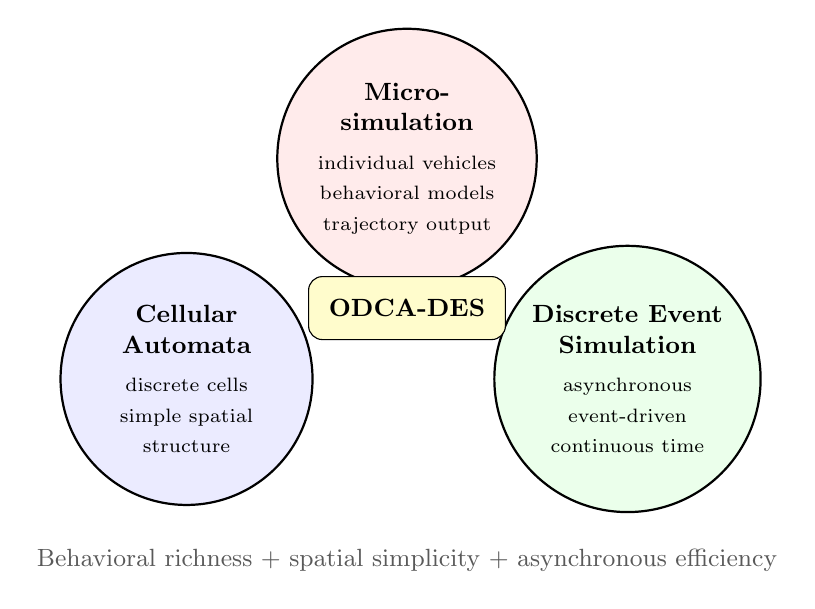
\begin{tikzpicture}[
    cir/.style={draw, circle, minimum size=3.2cm, thick, align=center, font=\small},
]
% Three overlapping circles (Venn-like)
\node[cir, fill=blue!8] (ca) at (-2.8,0) {\textbf{Cellular}\\  \textbf{Automata}\\[3pt] \scriptsize discrete cells\\  \scriptsize simple spatial\\  \scriptsize structure};
\node[cir, fill=green!8] (des) at (2.8,0) {\textbf{Discrete Event}\\  \textbf{Simulation}\\[3pt] \scriptsize asynchronous\\  \scriptsize event-driven\\  \scriptsize continuous time};
\node[cir, fill=red!8] (micro) at (0,2.8) {\textbf{Micro-}\\  \textbf{simulation}\\[3pt] \scriptsize individual vehicles\\  \scriptsize behavioral models\\  \scriptsize trajectory output};

% Center label
\node[draw, fill=yellow!20, rounded corners=5pt, font=\small\bfseries,
      minimum width=2.5cm, minimum height=0.8cm] (center) at (0,0.9) {ODCA-DES};

% Bottom tagline
\node[font=\small, text=gray!70!black] at (0,-2.3)
    {Behavioral richness $+$ spatial simplicity $+$ asynchronous efficiency};
\end{tikzpicture}
\end{center}
\end{frame}

% ==========================================================
\section{Traffic Flow Preliminaries}
% ==========================================================

% ----------------------------------------------------------
\begin{frame}{Trajectory Coordinates}
\begin{columns}[T]
\begin{column}{0.52\textwidth}
\begin{center}
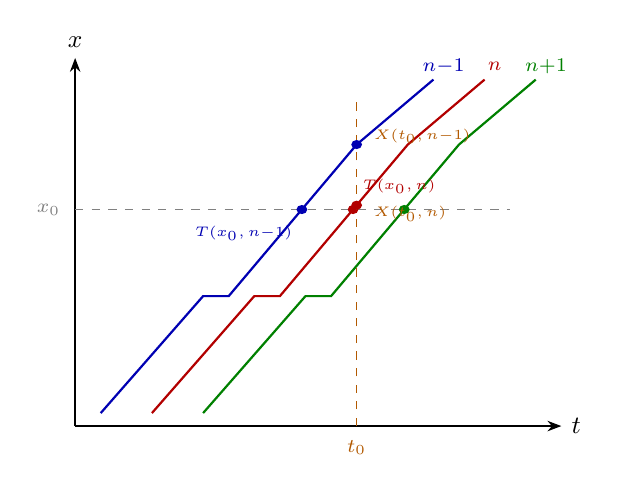
\begin{tikzpicture}[xscale=0.65, yscale=0.55]
% Axes
\draw[-{Stealth[length=5pt]}, thick] (0,0) -- (9.5,0) node[right, font=\small] {$t$};
\draw[-{Stealth[length=5pt]}, thick] (0,0) -- (0,8.5) node[above, font=\small] {$x$};

% Vehicle trajectories (5 vehicles, different slopes)
\draw[blue!70!black, thick] (0.5,0.3) -- (2.5,3.0) -- (3.0,3.0) -- (5.5,6.5) -- (7.0,8.0);
\draw[red!70!black, thick] (1.5,0.3) -- (3.5,3.0) -- (4.0,3.0) -- (6.5,6.5) -- (8.0,8.0);
\draw[green!50!black, thick] (2.5,0.3) -- (4.5,3.0) -- (5.0,3.0) -- (7.5,6.5) -- (9.0,8.0);

% Vehicle labels
\node[font=\scriptsize, blue!70!black] at (7.2,8.3) {$n{-}1$};
\node[font=\scriptsize, red!70!black] at (8.2,8.3) {$n$};
\node[font=\scriptsize, green!50!black] at (9.2,8.3) {$n{+}1$};

% T(x,n) annotation — horizontal line at position x_0
\draw[dashed, gray] (0,5.0) -- (8.5,5.0);
\node[font=\scriptsize, gray, anchor=east] at (-0.1,5.0) {$x_0$};
% Dots where trajectories cross x_0
\fill[blue!70!black] (4.43,5.0) circle (3pt);
\fill[red!70!black] (5.43,5.0) circle (3pt);
\fill[green!50!black] (6.43,5.0) circle (3pt);
% Labels near dots
\node[font=\tiny, blue!70!black, below left] at (4.43,4.85) {$T(x_0,n{-}1)$};
\node[font=\tiny, red!70!black, above right] at (5.43,5.15) {$T(x_0,n)$};

% X(t,n) annotation — vertical line at time t_0
\draw[dashed, orange!70!black] (5.5,0) -- (5.5,7.5);
\node[font=\scriptsize, orange!70!black, below] at (5.5,-0.1) {$t_0$};
% Dots
\fill[blue!70!black] (5.5,6.5) circle (3pt);
\fill[red!70!black] (5.5,5.1) circle (3pt);
% Labels near dots
\node[font=\tiny, orange!70!black, anchor=west] at (5.65,6.7) {$X(t_0,n{-}1)$};
\node[font=\tiny, orange!70!black, anchor=west] at (5.65,4.9) {$X(t_0,n)$};
\end{tikzpicture}
\end{center}
\end{column}
\begin{column}{0.45\textwidth}
\vspace{0.3em}
\textbf{Three coordinate systems:}

\vspace{0.5em}
{\small
\begin{tabular}{@{}cp{5.5cm}@{}}
$X(t,n)$ & Position of vehicle $n$ at time $t$ \\[6pt]
$T(x,n)$ & Time vehicle $n$ passes position $x$ \\[6pt]
$N(t,x)$ & Cumulative count of vehicles past $x$ by time $t$
\end{tabular}
}

\vspace{0.8em}
\begin{block}{Newell's Passage Time {\scriptsize(Newell, 1993, 2002 [1,2])}}
\vspace{0.2em}
$T(x,n)$ is the \textbf{inverse} of $X(t,n)$:\\[3pt]
{\small $X(t,n) = x_0 \;\Leftrightarrow\; T(x_0, n) = t$}
\end{block}

\vspace{0.5em}
{\small ODCA-DES outputs $T(x,n)$ \emph{natively}:\\
$\Tarr(c, i) \equiv T(c \cdot \ell,\; i)$}
\end{column}
\end{columns}
\end{frame}

% ----------------------------------------------------------
\begin{frame}{Traffic Flow Variables from Trajectories}
\begin{columns}[T]
\begin{column}{0.48\textwidth}
\vspace{0.3em}
\textbf{Point measurements} from $T(x,n)$:

\vspace{0.5em}
{\small
\renewcommand{\arraystretch}{1.6}
\begin{tabular}{@{}lc@{}}
Speed & $\displaystyle v_i(x) = \frac{\Delta x}{T(x{+}\Delta x, n) - T(x, n)}$ \\
Headway & $\displaystyle h(x) = T(x, n) - T(x, n{-}1)$ \\
Flow & $\displaystyle q(x) = \frac{1}{h(x)}$ \\
Spacing & $\displaystyle s(t) = X(t, n{-}1) - X(t, n)$ \\
Density & $\displaystyle k(t) = \frac{1}{s(t)}$
\end{tabular}
}

\vspace{0.6em}
\begin{alertblock}{Identity}
$q = k \cdot v$
\end{alertblock}
\end{column}
\begin{column}{0.50\textwidth}
\begin{center}
\textbf{Edie's generalized definitions} {\scriptsize(Edie, 1963 [8])}

\vspace{0.3em}
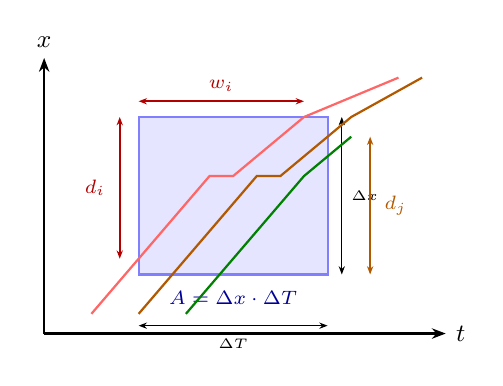
\begin{tikzpicture}[xscale=0.6, yscale=0.5]
% Axes
\draw[-{Stealth[length=5pt]}, thick] (0,0) -- (8.5,0) node[right, font=\small] {$t$};
\draw[-{Stealth[length=5pt]}, thick] (0,0) -- (0,7.0) node[above, font=\small] {$x$};

% Shaded rectangle
\fill[blue!10] (2,1.5) rectangle (6,5.5);
\draw[thick, blue!50] (2,1.5) rectangle (6,5.5);
\node[font=\scriptsize, blue!60!black] at (4,0.9) {$A = \Delta x \cdot \Delta T$};

% Dimension labels
\draw[{Stealth[length=3pt]}-{Stealth[length=3pt]}, thin] (2,0.2) -- (6,0.2);
\node[font=\tiny, below] at (4,0.1) {$\Delta T$};
\draw[{Stealth[length=3pt]}-{Stealth[length=3pt]}, thin] (6.3,1.5) -- (6.3,5.5);
\node[font=\tiny, right] at (6.3,3.5) {$\Delta x$};

% Trajectories through rectangle
\draw[red!60, thick] (1.0,0.5) -- (3.5,4.0) -- (4.0,4.0) -- (5.5,5.5) -- (7.5,6.5);
\draw[orange!70!black, thick] (2.0,0.5) -- (4.5,4.0) -- (5.0,4.0) -- (6.5,5.5) -- (8.0,6.5);
\draw[green!50!black, thick] (3.0,0.5) -- (5.5,4.0) -- (6.5,5.0);

% d_i annotation (vertical: distance traveled by red vehicle in region)
% Red enters rectangle at ~(2, 1.9), exits at (5.5, 5.5)
\draw[{Stealth[length=3pt]}-{Stealth[length=3pt]}, thick, red!70!black] (1.6,1.9) -- (1.6,5.5);
\node[font=\scriptsize, red!70!black, anchor=east] at (1.5,3.7) {$d_i$};

% w_i annotation (horizontal: time spent by red vehicle in region)
\draw[{Stealth[length=3pt]}-{Stealth[length=3pt]}, thick, red!70!black] (2,5.9) -- (5.5,5.9);
\node[font=\scriptsize, red!70!black, above] at (3.75,5.9) {$w_i$};

% d_j annotation (vertical: distance traveled by orange vehicle in region)
% Orange enters at ~(2.71, 1.5), exits at (6, 5.0)
\draw[{Stealth[length=3pt]}-{Stealth[length=3pt]}, thick, orange!70!black] (6.9,1.5) -- (6.9,5.0);
\node[font=\scriptsize, orange!70!black, anchor=west] at (7.0,3.25) {$d_j$};
\end{tikzpicture}
\end{center}

\vspace{-0.3em}
{\scriptsize $d_i$: distance by veh $i$, \; $w_i$: time spent by veh $i$}
{\small
\[
q = \frac{\sum d_i}{A}, \quad k = \frac{\sum w_i}{A}, \quad v = \frac{q}{k} = \frac{\sum d_i}{\sum w_i}
\]
}
\end{column}
\end{columns}
\end{frame}

% ----------------------------------------------------------
\begin{frame}{Kinematic Wave Model from Trajectories}
\begin{columns}[T]
\begin{column}{0.45\textwidth}
\begin{center}
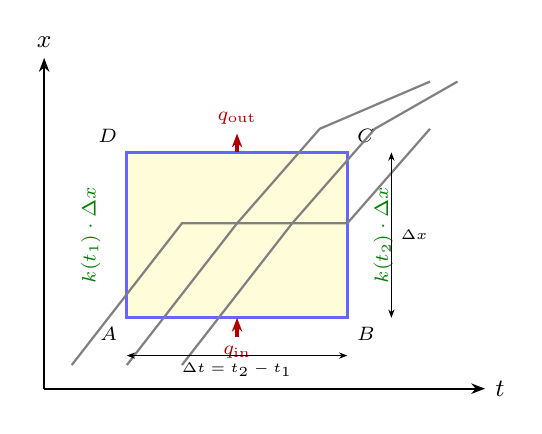
\begin{tikzpicture}[xscale=0.7, yscale=0.6]
% Axes
\draw[-{Stealth[length=5pt]}, thick] (0,0) -- (8.0,0) node[right, font=\small] {$t$};
\draw[-{Stealth[length=5pt]}, thick] (0,0) -- (0,7.0) node[above, font=\small] {$x$};

% Rectangle ABCD
\fill[yellow!15] (1.5,1.5) rectangle (5.5,5.0);
\draw[very thick, blue!60] (1.5,1.5) rectangle (5.5,5.0);

% Corner labels
\node[font=\scriptsize, anchor=north east] at (1.5,1.5) {$A$};
\node[font=\scriptsize, anchor=north west] at (5.5,1.5) {$B$};
\node[font=\scriptsize, anchor=south west] at (5.5,5.0) {$C$};
\node[font=\scriptsize, anchor=south east] at (1.5,5.0) {$D$};

% Flow arrows on sides
\draw[-{Stealth[length=5pt]}, very thick, red!70!black] (3.5,1.1) -- (3.5,1.5);
\node[font=\scriptsize, red!70!black, below] at (3.5,1.1) {$q_{\text{in}}$};
\draw[-{Stealth[length=5pt]}, very thick, red!70!black] (3.5,5.0) -- (3.5,5.4);
\node[font=\scriptsize, red!70!black, above] at (3.5,5.4) {$q_{\text{out}}$};

% Density labels on sides
\node[font=\scriptsize, green!50!black, rotate=90, anchor=south] at (1.2,3.25) {$k(t_1) \cdot \Delta x$};
\node[font=\scriptsize, green!50!black, rotate=90, anchor=north] at (5.8,3.25) {$k(t_2) \cdot \Delta x$};

% Trajectories passing through
\draw[gray, thick] (0.5,0.5) -- (2.5,3.5) -- (3.5,3.5) -- (5.0,5.5) -- (7.0,6.5);
\draw[gray, thick] (1.5,0.5) -- (3.5,3.5) -- (4.5,3.5) -- (6.0,5.5) -- (7.5,6.5);
\draw[gray, thick] (2.5,0.5) -- (4.5,3.5) -- (5.5,3.5) -- (7.0,5.5);

% Dimension annotations
\draw[{Stealth[length=3pt]}-{Stealth[length=3pt]}, thin] (1.5,0.7) -- (5.5,0.7);
\node[font=\tiny] at (3.5,0.4) {$\Delta t = t_2 - t_1$};
\draw[{Stealth[length=3pt]}-{Stealth[length=3pt]}, thin] (6.3,1.5) -- (6.3,5.0);
\node[font=\tiny, right] at (6.3,3.25) {$\Delta x$};
\end{tikzpicture}
\end{center}
\end{column}
\begin{column}{0.52\textwidth}
\vspace{0.3em}
\textbf{Conservation of vehicles} in rectangle:

\vspace{0.3em}
{\small
vehicles in at $t_2$ $-$ vehicles in at $t_1$\\
$=$ vehicles entering from bottom $-$ leaving from top
}

\vspace{0.3em}
\[
k(x, t_2)\,\Delta x - k(x, t_1)\,\Delta x = \big[q(x_1, t) - q(x_2, t)\big]\,\Delta t
\]

\vspace{0.3em}
Divide by $\Delta x \cdot \Delta t$ and take limits:

\vspace{0.1em}
\[
\boxed{\frac{\partial k}{\partial t} + \frac{\partial q}{\partial x} = 0}
\]

\vspace{0.3em}
\textbf{LWR kinematic wave equation}\\[3pt]
{\scriptsize (Lighthill--Whitham 1955, Richards 1956)}

\vspace{0.5em}
With $q = Q(k)$ (fundamental diagram):
\[
\frac{\partial k}{\partial t} + Q'(k)\frac{\partial k}{\partial x} = 0
\]

{\small Waves propagate at speed $c = Q'(k) = dq/dk$}

\vspace{0.3em}
\begin{exampleblock}{\small Triangular FD}
{\scriptsize Free flow: $c = v_f$, \; Congested: $c = -w = -\ell/\tau$}
\end{exampleblock}
\end{column}
\end{columns}
\end{frame}

% ----------------------------------------------------------
\begin{frame}[shrink=12]{Triangular Fundamental Diagram}
\begin{columns}[T]
\begin{column}{0.55\textwidth}
\begin{center}
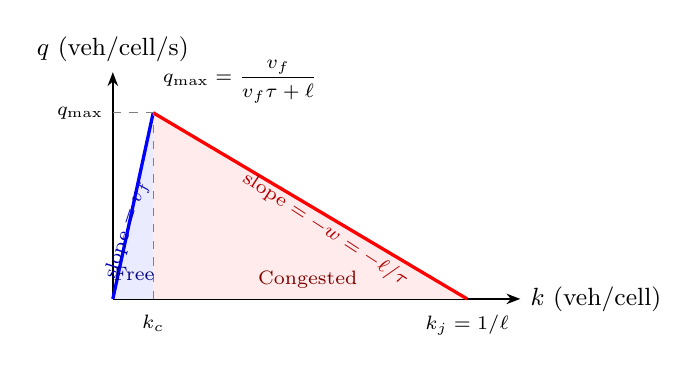
\begin{tikzpicture}[xscale=4.5, yscale=4.0]
% Axes
\draw[-{Stealth[length=5pt]}, thick] (0,0) -- (1.15,0) node[right, font=\small] {$k$ (veh/cell)};
\draw[-{Stealth[length=5pt]}, thick] (0,0) -- (0,0.72) node[above, font=\small] {$q$ (veh/cell/s)};

% Shaded regions
\fill[blue!8] (0,0) -- (0.114,0.591) -- (0.114,0) -- cycle;
\fill[red!8] (0.114,0) -- (0.114,0.591) -- (1.0,0) -- cycle;

% FD lines
\draw[blue, very thick] (0,0) -- (0.114,0.591);
\draw[red, very thick] (0.114,0.591) -- (1.0,0);

% Labels
\node[font=\scriptsize, above right] at (0.114,0.591) {$q_{\max} = \dfrac{v_f}{v_f \tau + \ell}$};
\draw[dashed, thin, gray] (0.114,0) -- (0.114,0.591);
\draw[dashed, thin, gray] (0,0.591) -- (0.114,0.591);
\node[font=\scriptsize, below] at (0.114,-0.02) {$k_c$};
\node[font=\scriptsize, below] at (1.0,-0.02) {$k_j = 1/\ell$};
\node[font=\scriptsize, left] at (0,0.591) {$q_{\max}$};

% Regime labels
\node[font=\scriptsize, blue!70!black, rotate=72] at (0.04,0.22) {slope $= v_f$};
\node[font=\scriptsize, red!70!black, rotate=-33] at (0.6,0.22) {slope $= -w = -\ell/\tau$};

% Region labels
\node[font=\scriptsize, blue!50!black] at (0.06,0.08) {Free};
\node[font=\scriptsize, red!50!black] at (0.55,0.06) {Congested};
\end{tikzpicture}
\end{center}
\end{column}
\begin{column}{0.42\textwidth}
\vspace{0.5em}
Emerges from \textbf{two parameters}:

\vspace{0.5em}
{\small
\begin{tabular}{@{}ll@{}}
Cell length & $\ell = 7.5$\,m \\
Release delay & $\tau = 1.5$\,s \\
\midrule
$v_f$ & $5.2$\,cells/s (140\,km/h) \\
$q_{\max}$ & 2127\,veh/h \\
$w$ & 18\,km/h \\
$k_j$ & 133\,veh/km \\
\end{tabular}
}

\vspace{0.8em}
\begin{block}{Key Result}
Identical to Newell's kinematic wave model.

\vspace{0.3em}
\alert{No FD calibration needed} --- it is an inherent consequence of the resource protocol.
\end{block}
\end{column}
\end{columns}
\end{frame}

% ==========================================================
\section{ODCA-DES Framework}
% ==========================================================

% ----------------------------------------------------------
\begin{frame}[shrink=15]{Framework Architecture}
\begin{center}
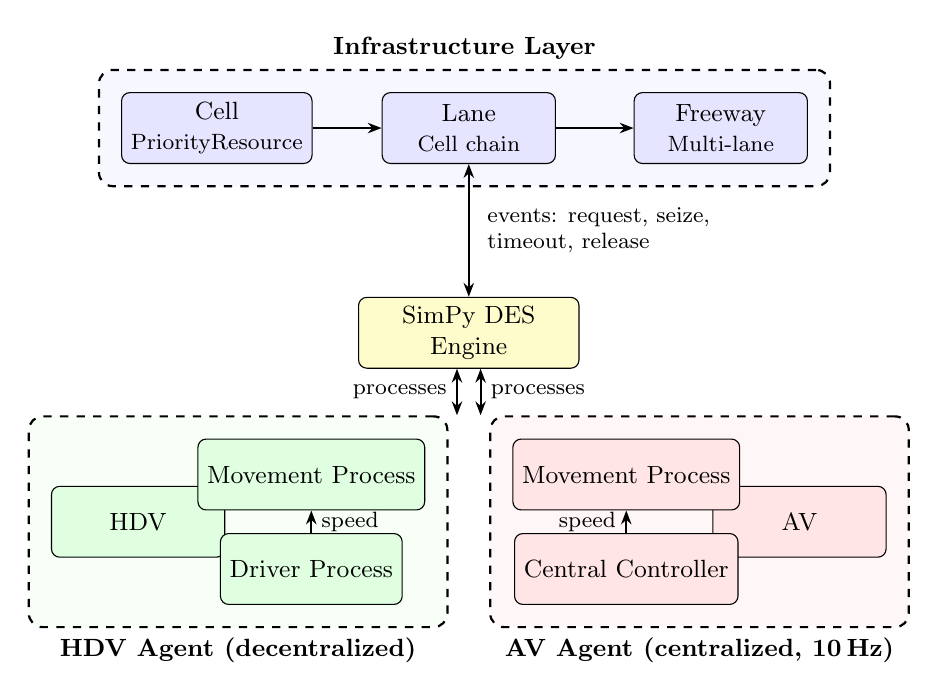
\begin{tikzpicture}[
    box/.style={draw, rounded corners=3pt, minimum width=2.2cm, minimum height=0.9cm,
                align=center, font=\small},
    bigbox/.style={draw, rounded corners=5pt, inner sep=8pt, dashed, thick},
    arr/.style={-{Stealth[length=5pt]}, thick},
    darr/.style={{Stealth[length=5pt]}-{Stealth[length=5pt]}, thick},
]
% Infrastructure layer
\node[box, fill=blue!10] (lane) at (0,0) {Lane\\{\footnotesize Cell chain}};
\node[box, fill=blue!10] (cell) at (-3.2,0) {Cell\\{\footnotesize PriorityResource}};
\node[box, fill=blue!10] (freeway) at (3.2,0) {Freeway\\{\footnotesize Multi-lane}};
\draw[arr] (cell) -- (lane);
\draw[arr] (lane) -- (freeway);

% DES Engine
\node[box, fill=yellow!20, minimum width=2.8cm] (engine) at (0,-2.6) {SimPy DES\\Engine};

% HDV Agent
\node[box, fill=green!12] (hdv) at (-4.2,-5.0) {HDV};
\node[box, fill=green!12] (mvmt) at (-2.0,-4.4) {Movement Process};
\node[box, fill=green!12] (driver) at (-2.0,-5.6) {Driver Process};
\draw[arr] (driver) -- node[right, font=\footnotesize] {speed} (mvmt);

% AV Agent
\node[box, fill=red!10] (av) at (4.2,-5.0) {AV};
\node[box, fill=red!10] (avmvmt) at (2.0,-4.4) {Movement Process};
\node[box, fill=red!10] (ctrl) at (2.0,-5.6) {Central Controller};
\draw[arr] (ctrl) -- node[left, font=\footnotesize] {speed} (avmvmt);

% Grouping boxes
\begin{scope}[on background layer]
    \node[bigbox, fill=blue!3, fit=(cell)(lane)(freeway),
          label={[font=\small\bfseries]above:Infrastructure Layer}] (infra) {};
    \node[bigbox, fill=green!3, fit=(hdv)(mvmt)(driver),
          label={[font=\small\bfseries]below:HDV Agent (decentralized)}] (hdvbox) {};
    \node[bigbox, fill=red!3, fit=(av)(avmvmt)(ctrl),
          label={[font=\small\bfseries]below:AV Agent (centralized, 10\,Hz)}] (avbox) {};
\end{scope}

% Arrows
\draw[darr] (engine.north) -- node[right, font=\footnotesize, align=left, xshift=3pt]
    {events: request, seize,\\timeout, release} (lane.south);

\coordinate (eng_bl) at ($(engine.south) + (-0.15,0)$);
\coordinate (eng_br) at ($(engine.south) + (0.15,0)$);
\draw[darr] (eng_bl) -- node[left, font=\footnotesize] {processes} (eng_bl |- hdvbox.north);
\draw[darr] (eng_br) -- node[right, font=\footnotesize] {processes} (eng_br |- avbox.north);
\end{tikzpicture}
\end{center}
\end{frame}

% ----------------------------------------------------------
\begin{frame}[shrink=15]{Newell's Simplified Car-Following Model}
\begin{columns}[T]
\begin{column}{0.52\textwidth}
\begin{center}
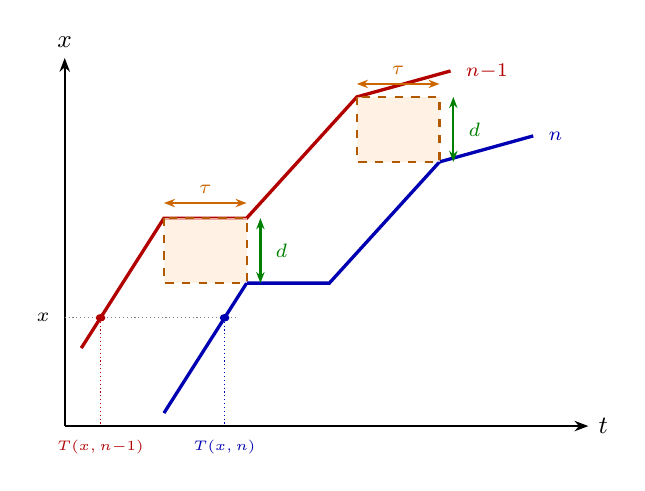
\begin{tikzpicture}[xscale=0.7, yscale=0.55]
% Axes
\draw[-{Stealth[length=5pt]}, thick] (0,0) -- (9.5,0) node[right, font=\small] {$t$};
\draw[-{Stealth[length=5pt]}, thick] (0,0) -- (0,8.5) node[above, font=\small] {$x$};

% Leader trajectory (higher up, more separation)
\draw[red!70!black, very thick] (0.3,1.8) -- (1.8,4.8) -- (3.3,4.8) -- (5.3,7.6) -- (7.0,8.2);
\node[font=\scriptsize, red!70!black, anchor=west] at (7.1,8.2) {$n{-}1$};

% Follower trajectory (shifted by tau=1.5 in time, d=1.5 in space)
\draw[blue!70!black, very thick] (1.8,0.3) -- (3.3,3.3) -- (4.8,3.3) -- (6.8,6.1) -- (8.5,6.7);
\node[font=\scriptsize, blue!70!black, anchor=west] at (8.6,6.7) {$n$};

% --- First (tau, d) rectangle at the stop region ---
% Leader is at (1.8, 4.8), follower arrives at corresponding point (3.3, 3.3)
% Rectangle corners: leader point -> (+tau, 0) -> (+tau, -d) -> (0, -d)
\fill[orange!15, opacity=0.7] (1.8,4.8) rectangle (3.3,3.3);
\draw[orange!70!black, thick, dashed] (1.8,4.8) rectangle (3.3,3.3);

% tau arrow (top edge of rectangle)
\draw[{Stealth[length=4pt]}-{Stealth[length=4pt]}, thick, orange!80!black]
    (1.8,5.15) -- (3.3,5.15);
\node[font=\scriptsize, orange!80!black, above] at (2.55,5.15) {$\tau$};

% d arrow (right edge of rectangle)
\draw[{Stealth[length=4pt]}-{Stealth[length=4pt]}, thick, green!50!black]
    (3.55,3.3) -- (3.55,4.8);
\node[font=\scriptsize, green!50!black, anchor=west] at (3.65,4.05) {$d$};

% --- Second (tau, d) rectangle in the moving region ---
% Leader at (5.3, 7.6), follower at (6.8, 6.1)
\fill[orange!15, opacity=0.7] (5.3,7.6) rectangle (6.8,6.1);
\draw[orange!70!black, thick, dashed] (5.3,7.6) rectangle (6.8,6.1);

% tau arrow
\draw[{Stealth[length=4pt]}-{Stealth[length=4pt]}, thick, orange!80!black]
    (5.3,7.9) -- (6.8,7.9);
\node[font=\scriptsize, orange!80!black, above] at (6.05,7.9) {$\tau$};

% d arrow
\draw[{Stealth[length=4pt]}-{Stealth[length=4pt]}, thick, green!50!black]
    (7.05,6.1) -- (7.05,7.6);
\node[font=\scriptsize, green!50!black, anchor=west] at (7.15,6.85) {$d$};

% --- Passage time annotation ---
% Horizontal line at x = 2.5
\draw[thin, densely dotted, gray] (0,2.5) -- (3.1,2.5);
\node[font=\scriptsize, anchor=east] at (-0.1,2.5) {$x$};
% Leader crosses x=2.5 at t≈0.65 (segment 0.3,1.8 -- 1.8,4.8)
\fill[red!70!black] (0.65,2.5) circle (2.5pt);
\draw[thin, densely dotted, red!70!black] (0.65,2.5) -- (0.65,0);
\node[font=\tiny, red!70!black, below] at (0.65,-0.1) {$T(x,n{-}1)$};
% Follower crosses x=2.5 at t≈2.9 (segment 1.8,0.3 -- 3.3,3.3)
\fill[blue!70!black] (2.9,2.5) circle (2.5pt);
\draw[thin, densely dotted, blue!70!black] (2.9,2.5) -- (2.9,0);
\node[font=\tiny, blue!70!black, below] at (2.9,-0.1) {$T(x,n)$};
\end{tikzpicture}
\end{center}
{\scriptsize Follower = leader shifted by $(\tau, d)$; shaded rectangle is constant between corresponding points}
\end{column}
\begin{column}{0.45\textwidth}
\vspace{0.5em}
\textbf{Position form:}
\[
X_{n}(t) = X_{n-1}(t - \tau) - d
\]

\vspace{0.3em}
\textbf{Passage-time form:}
\[
\boxed{T(x, n) = T(x + d,\; n{-}1) + \tau}
\]
{\scriptsize Vehicle $n$ passes position $x$ exactly $\tau$\,s after its leader passed $x{+}d$}

\vspace{0.8em}
{\small
\begin{tabular}{@{}ll@{}}
$\tau$ & reaction time (s) \\
$d$ & standstill spacing (m) \\
$v_f$ & free-flow speed \\
\end{tabular}
}

\vspace{0.8em}
\begin{block}{Triangular FD}
$q_{\max} = \dfrac{v_f}{v_f \tau + d}$
\qquad $w = \dfrac{d}{\tau}$
\end{block}
\end{column}
\end{columns}
\end{frame}

% ----------------------------------------------------------
\begin{frame}{Why Newell? A Natural Fit for ODCA-DES}
\begin{center}
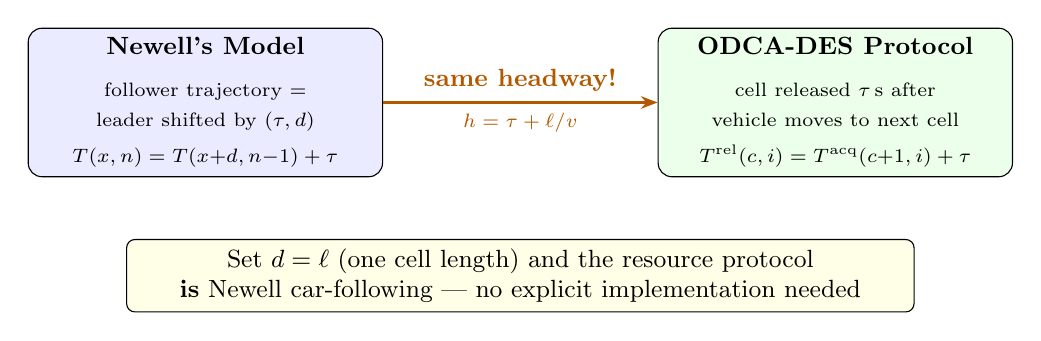
\begin{tikzpicture}[
    box/.style={draw, rounded corners=5pt, minimum width=4.5cm, minimum height=1.8cm,
                align=center, font=\small},
    arr/.style={-{Stealth[length=6pt]}, very thick},
]
% Newell box
\node[box, fill=blue!8] (newell) at (-4, 0) {
    \textbf{Newell's Model}\\[4pt]
    {\scriptsize follower trajectory =}\\
    {\scriptsize leader shifted by $(\tau, d)$}\\[2pt]
    {\scriptsize $T(x,n) = T(x{+}d, n{-}1) + \tau$}
};

% ODCA-DES box
\node[box, fill=green!8] (odca) at (4, 0) {
    \textbf{ODCA-DES Protocol}\\[4pt]
    {\scriptsize cell released $\tau$\,s after}\\
    {\scriptsize vehicle moves to next cell}\\[2pt]
    {\scriptsize $\Trel(c,i) = \Tacq(c{+}1,i) + \tau$}
};

% Equivalence arrow
\draw[arr, orange!70!black] (newell) -- (odca)
    node[midway, above, font=\small\bfseries, orange!70!black] {same headway!}
    node[midway, below, font=\scriptsize] {$h = \tau + \ell/v$};

% Bottom annotations
\node[draw, rounded corners=3pt, fill=yellow!10, font=\small, align=center,
      minimum width=10cm] at (0, -2.2)
    {Set $d = \ell$ (one cell length) and the resource protocol\\
     \textbf{is} Newell car-following --- no explicit implementation needed};
\end{tikzpicture}
\end{center}
\end{frame}

% ----------------------------------------------------------
\begin{frame}{Hybrid Discretization: Three Dimensions}
\begin{center}
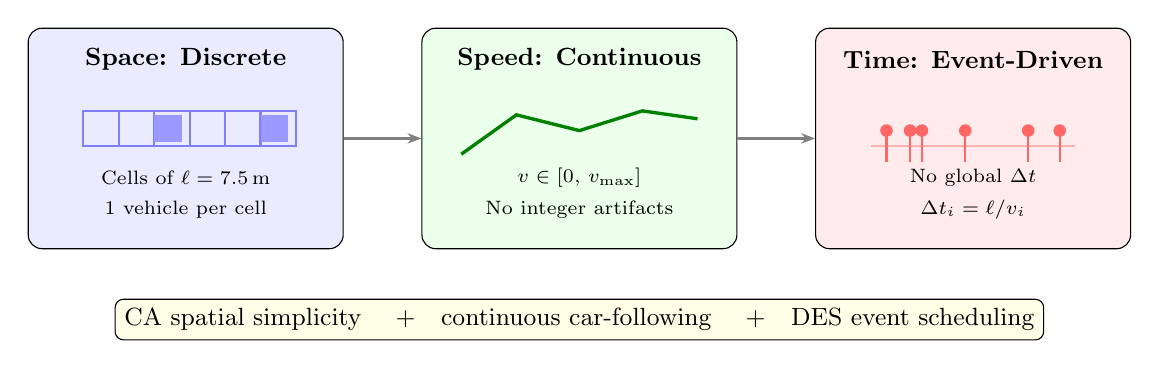
\begin{tikzpicture}[
    dimbox/.style={draw, rounded corners=5pt, minimum width=4.0cm, minimum height=2.8cm,
                   align=center, font=\small},
]
% Space
\node[dimbox, fill=blue!8] (sp) at (-5,0) {};
\node[font=\small\bfseries] at (-5,1.0) {Space: Discrete};
% Draw cells
\foreach \x in {0,...,5} {
    \draw[thick, blue!50] (-6.3+\x*0.45, -0.1) rectangle (-5.85+\x*0.45, 0.35);
}
% Car in one cell
\fill[blue!40] (-5.85+1*0.45, -0.05) rectangle (-5.85+1*0.45+0.35, 0.3);
\fill[blue!40] (-5.85+4*0.45, -0.05) rectangle (-5.85+4*0.45+0.35, 0.3);
\node[font=\scriptsize] at (-5,-0.5) {Cells of $\ell = 7.5$\,m};
\node[font=\scriptsize] at (-5,-0.9) {1 vehicle per cell};

% Speed
\node[dimbox, fill=green!8] (vel) at (0,0) {};
\node[font=\small\bfseries] at (0,1.0) {Speed: Continuous};
% Draw smooth curve
\draw[very thick, green!50!black] (-1.5,-0.2) -- (-0.8,0.3) -- (0,0.1) -- (0.8,0.35) -- (1.5,0.25);
\node[font=\scriptsize] at (0,-0.5) {$v \in [0,\, v_{\max}]$};
\node[font=\scriptsize] at (0,-0.9) {No integer artifacts};

% Time
\node[dimbox, fill=red!8] (tm) at (5,0) {};
\node[font=\small\bfseries] at (5,1.0) {Time: Event-Driven};
% Draw timeline with uneven events
\draw[thick, red!30] (3.7,-0.1) -- (6.3,-0.1);
\foreach \x/\w in {3.9/0.08, 4.2/0.08, 4.35/0.08, 4.9/0.08, 5.7/0.08, 6.1/0.08} {
    \draw[thick, red!60] (\x,-0.3) -- (\x,0.1);
    \fill[red!60] (\x,0.1) circle (\w);
}
\node[font=\scriptsize] at (5,-0.5) {No global $\Delta t$};
\node[font=\scriptsize] at (5,-0.9) {$\Delta t_i = \ell / v_i$};

% Arrows connecting
\draw[-{Stealth[length=5pt]}, thick, gray] (sp) -- (vel);
\draw[-{Stealth[length=5pt]}, thick, gray] (vel) -- (tm);

% Bottom summary
\node[draw, rounded corners=3pt, fill=yellow!10, font=\small, align=center] at (0,-2.3)
    {CA spatial simplicity \quad$+$\quad continuous car-following \quad$+$\quad DES event scheduling};
\end{tikzpicture}
\end{center}
\end{frame}

% ----------------------------------------------------------
\begin{frame}{Hybrid Discretization: Microsim vs.\ CA vs.\ ODCA}
\begin{center}
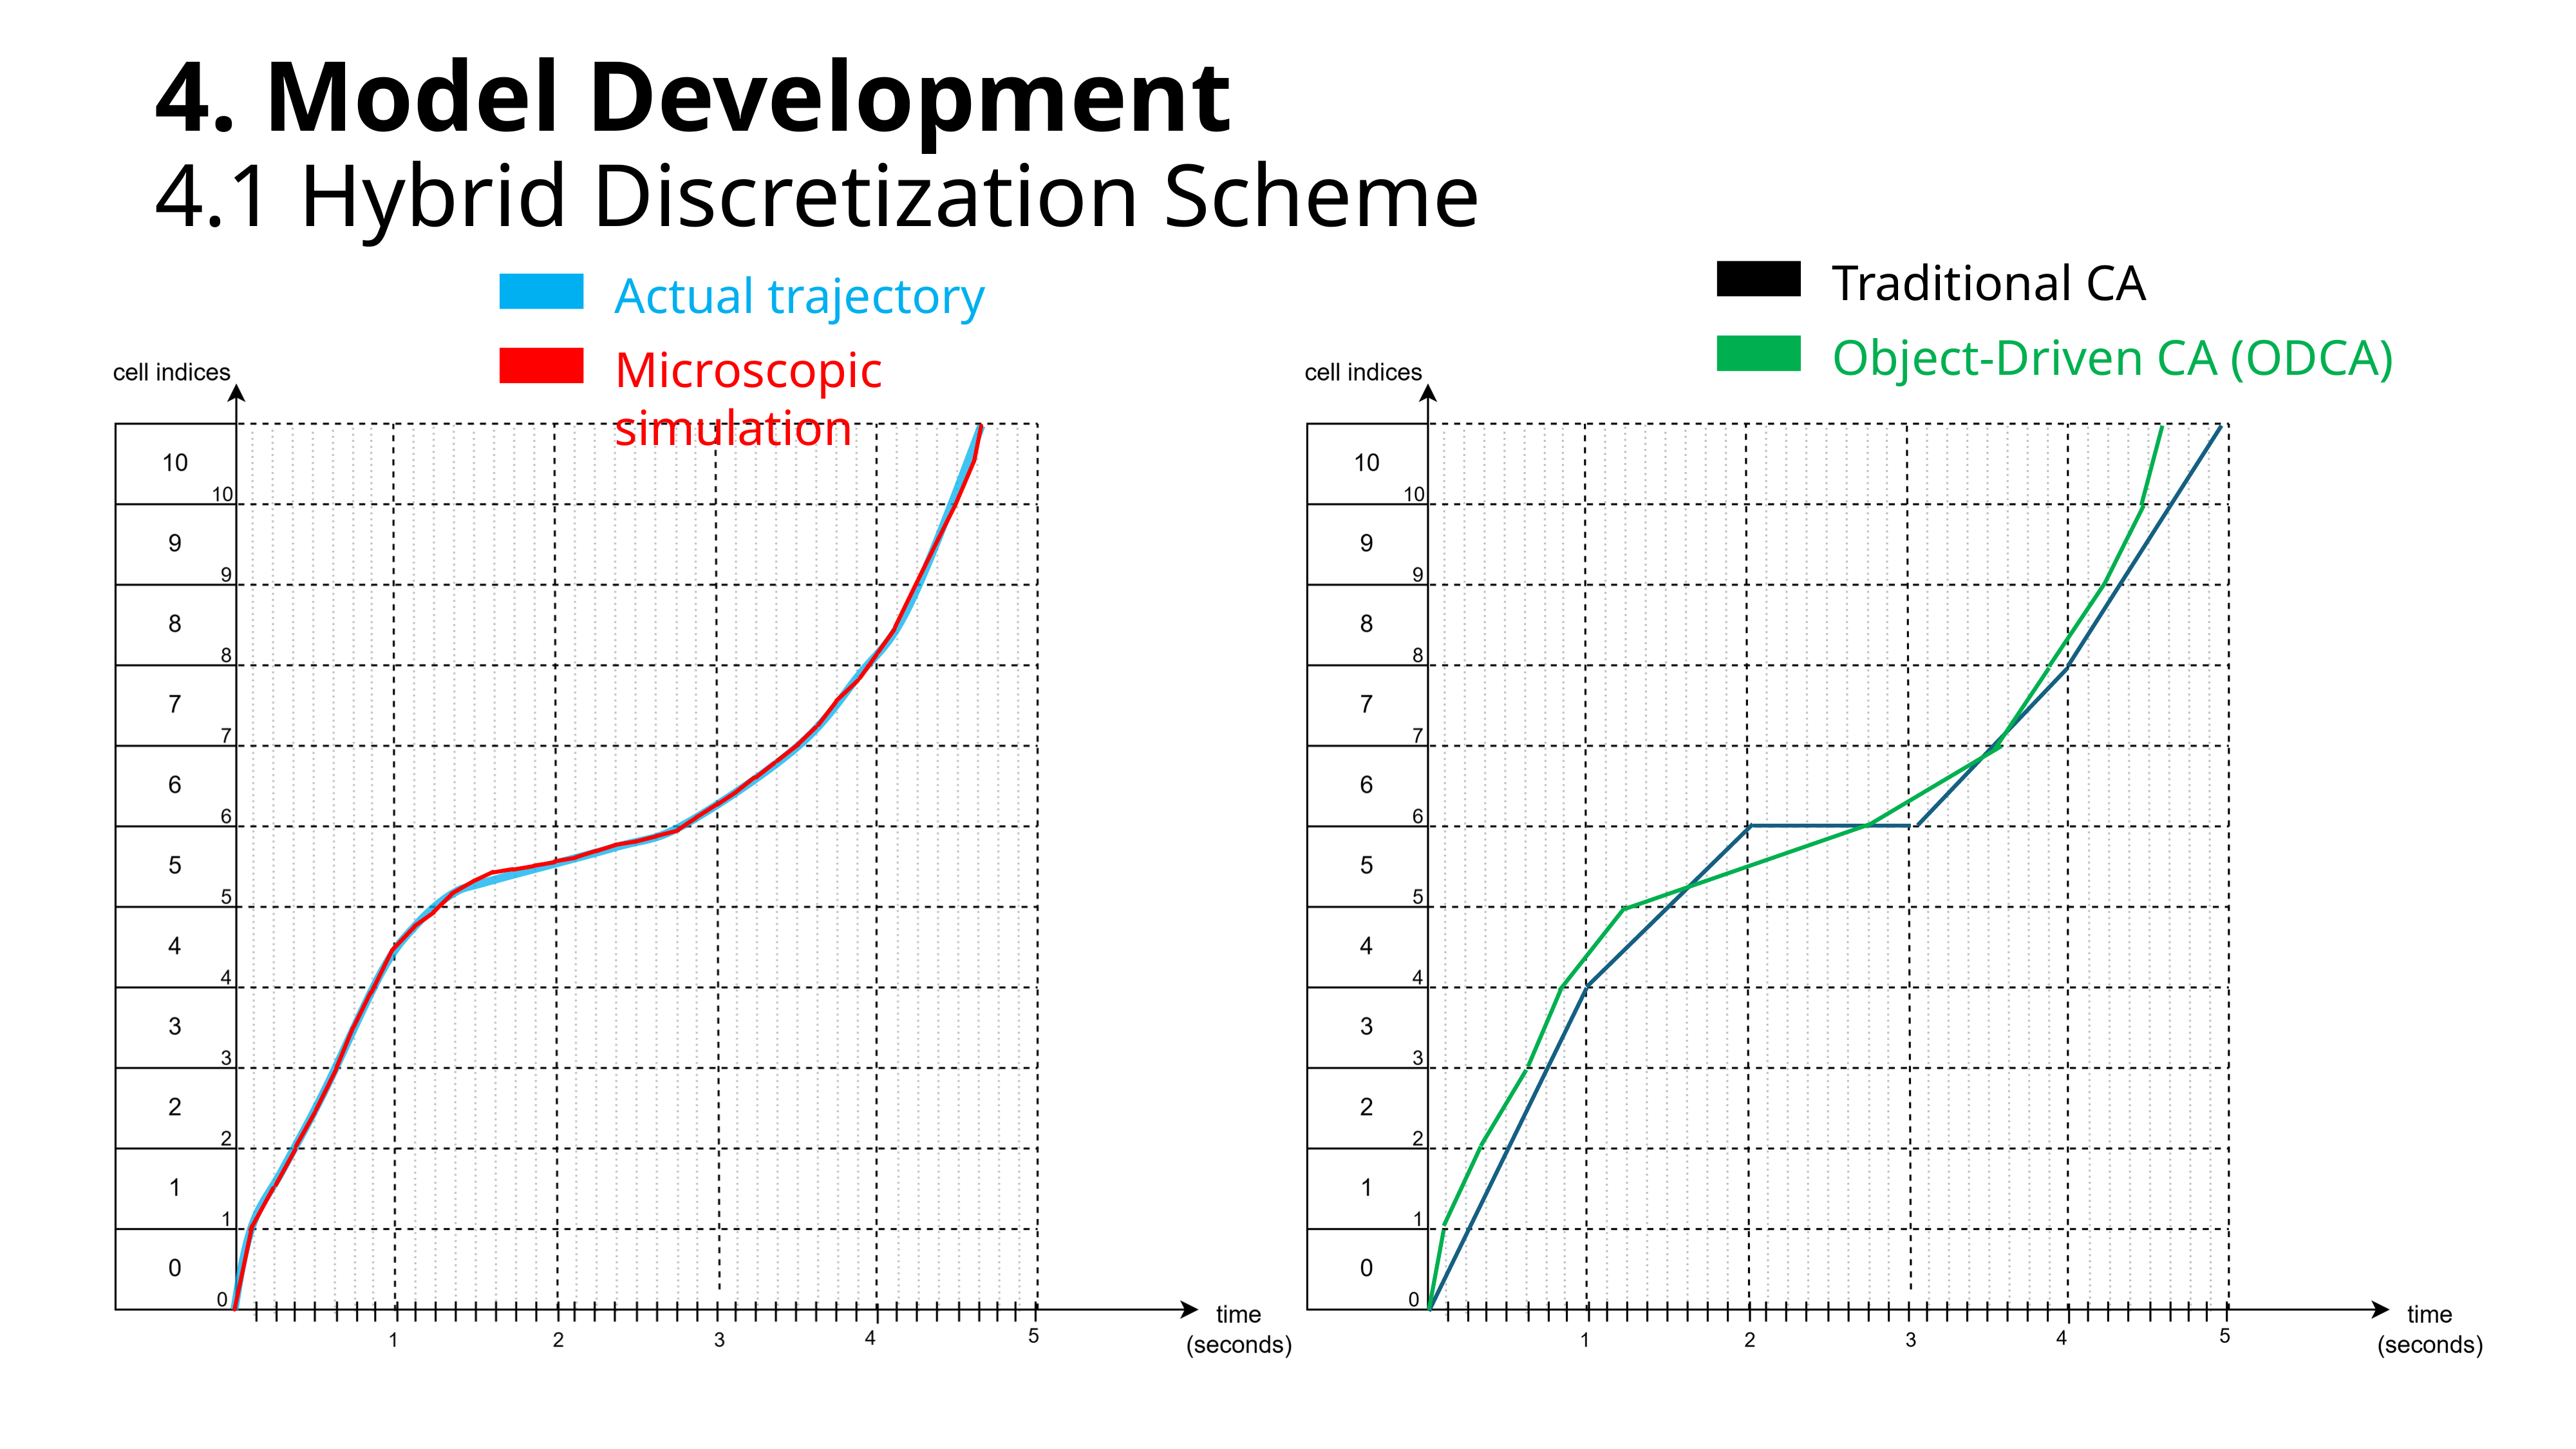
\includegraphics[width=0.92\textwidth,height=0.82\textheight,keepaspectratio]{diss_slide13-13.png}
\end{center}
\vspace{-0.5em}
{\small \textbf{Left:} Microsim closely tracks actual trajectory.
\textbf{Right:} ODCA records cell-crossing times (continuous), traditional CA uses integer steps.}
\end{frame}

% ----------------------------------------------------------
\begin{frame}{Infrastructure Model}
\begin{center}
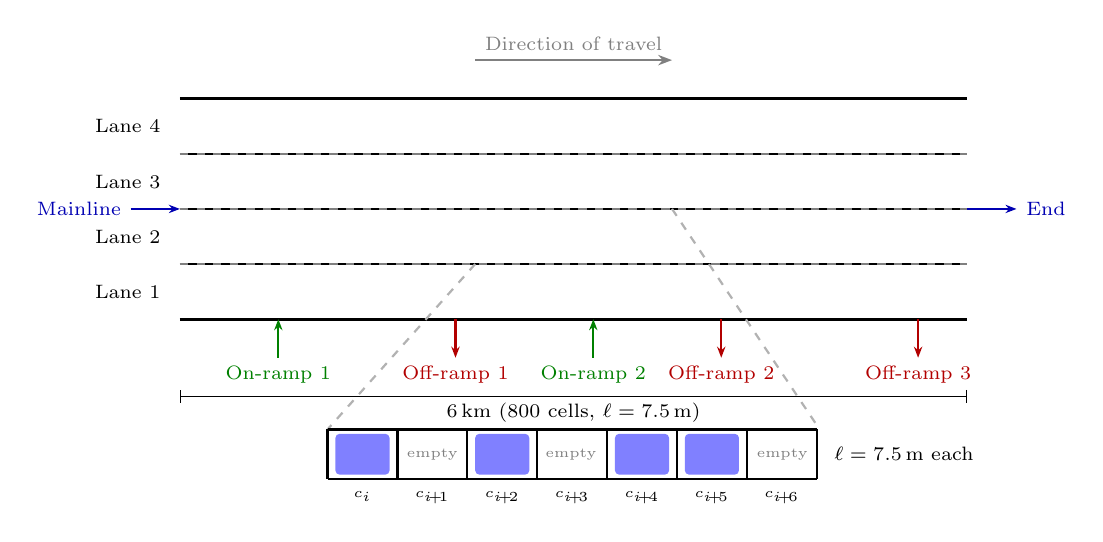
\begin{tikzpicture}[
    x=1.25cm, y=0.7cm,
    ramp/.style={-{Stealth[length=4pt]}, thick},
    lbl/.style={font=\scriptsize},
]
% Freeway lanes
\foreach \y in {0,1,2,3,4} {
    \draw[thick] (0,\y) -- (8,\y);
}
\foreach \y in {1,2,3} {
    \draw[thick, dashed, gray] (0,\y) -- (8,\y);
}
\draw[very thick] (0,0) -- (8,0);
\draw[very thick] (0,4) -- (8,4);

\node[lbl, anchor=east] at (-0.1,0.5) {Lane 1};
\node[lbl, anchor=east] at (-0.1,1.5) {Lane 2};
\node[lbl, anchor=east] at (-0.1,2.5) {Lane 3};
\node[lbl, anchor=east] at (-0.1,3.5) {Lane 4};

\draw[ramp, blue!70!black] (-0.5,2) -- (0,2);
\node[lbl, blue!70!black, anchor=east] at (-0.5,2) {Mainline};
\draw[ramp, blue!70!black] (8,2) -- (8.5,2);
\node[lbl, blue!70!black, anchor=west] at (8.5,2) {End};

\draw[ramp, green!50!black] (1.0,-0.7) -- (1.0,0);
\node[lbl, green!50!black] at (1.0,-1.0) {On-ramp 1};

\draw[ramp, green!50!black] (4.2,-0.7) -- (4.2,0);
\node[lbl, green!50!black] at (4.2,-1.0) {On-ramp 2};

\draw[ramp, red!70!black] (2.8,0) -- (2.8,-0.7);
\node[lbl, red!70!black] at (2.8,-1.0) {Off-ramp 1};

\draw[ramp, red!70!black] (5.5,0) -- (5.5,-0.7);
\node[lbl, red!70!black] at (5.5,-1.0) {Off-ramp 2};

\draw[ramp, red!70!black] (7.5,0) -- (7.5,-0.7);
\node[lbl, red!70!black] at (7.5,-1.0) {Off-ramp 3};

\draw[|-|, thin] (0,-1.4) -- (8,-1.4);
\node[lbl] at (4,-1.7) {6\,km (800 cells, $\ell = 7.5$\,m)};

\draw[-{Stealth[length=5pt]}, thick, gray] (3,4.7) -- (5,4.7);
\node[lbl, gray, above] at (4,4.7) {Direction of travel};

% --- Zoom inset: cells below freeway ---
% Zoom lines from a section of Lane 2
\draw[dashed, gray!60, thick] (3.0,1) -- (1.5,-2.0);
\draw[dashed, gray!60, thick] (5.0,2) -- (6.5,-2.0);
% Cell grid (centered below freeway)
\foreach \x in {0,...,7} {
    \draw[thick] (1.5+\x*0.71,-2.0) -- (1.5+\x*0.71,-2.9);
}
\draw[thick] (1.5,-2.0) -- (6.47,-2.0);
\draw[thick] (1.5,-2.9) -- (6.47,-2.9);
% Vehicles in some cells (blue rectangles, inset within cell boundaries)
% Cell boundaries: c_i=1.50..2.21, c_{i+1}=2.21..2.92, c_{i+2}=2.92..3.63,
%   c_{i+3}=3.63..4.34, c_{i+4}=4.34..5.05, c_{i+5}=5.05..5.76, c_{i+6}=5.76..6.47
% Pad 0.08 from each cell wall
\fill[blue!50, rounded corners=1.5pt] (1.58,-2.82) rectangle (2.13,-2.08);  % c_i
\fill[blue!50, rounded corners=1.5pt] (3.00,-2.82) rectangle (3.55,-2.08);  % c_{i+2}
\fill[blue!50, rounded corners=1.5pt] (4.42,-2.82) rectangle (4.97,-2.08);  % c_{i+4}
\fill[blue!50, rounded corners=1.5pt] (5.13,-2.82) rectangle (5.68,-2.08);  % c_{i+5}
% Empty cell labels
\node[font=\tiny, gray] at (2.565,-2.45) {empty};
\node[font=\tiny, gray] at (3.975,-2.45) {empty};
\node[font=\tiny, gray] at (6.12,-2.45) {empty};
% Cell labels
\node[lbl, below] at (1.855,-2.95) {\tiny $c_i$};
\node[lbl, below] at (2.565,-2.95) {\tiny $c_{i\!+\!1}$};
\node[lbl, below] at (3.275,-2.95) {\tiny $c_{i\!+\!2}$};
\node[lbl, below] at (3.985,-2.95) {\tiny $c_{i\!+\!3}$};
\node[lbl, below] at (4.695,-2.95) {\tiny $c_{i\!+\!4}$};
\node[lbl, below] at (5.405,-2.95) {\tiny $c_{i\!+\!5}$};
\node[lbl, below] at (6.115,-2.95) {\tiny $c_{i\!+\!6}$};
\node[lbl, right] at (6.55,-2.45) {\scriptsize $\ell = 7.5$\,m each};
\end{tikzpicture}
\end{center}

\vspace{0.3em}
\centering
{\small Each \textbf{cell} = SimPy PriorityResource (capacity 1) --- at most one vehicle per cell}
\end{frame}

% ----------------------------------------------------------
\begin{frame}{Movement Protocol: The Core Mechanism}
\begin{center}
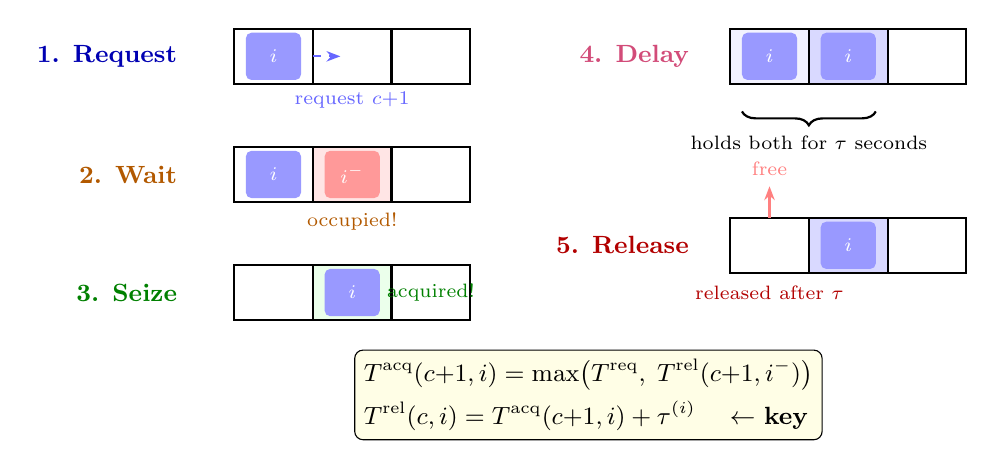
\begin{tikzpicture}[
    cell/.style={draw, thick, minimum width=1.0cm, minimum height=0.7cm, font=\small},
    arr/.style={-{Stealth[length=5pt]}, thick},
]
% --- Step 1: Request ---
\node[font=\small\bfseries, blue!70!black, anchor=east] at (-4.1, 2.3) {1. Request};
\node[cell] at (-3.0, 2.3) {};
\node[cell] at (-2.0, 2.3) {};
\node[cell] at (-1.0, 2.3) {};
\fill[blue!40, rounded corners=2pt] (-3.35,2.0) rectangle (-2.65,2.6);
\node[font=\scriptsize, white] at (-3.0,2.3) {$i$};
\draw[arr, blue!60, dashed] (-2.5,2.3) -- (-2.15,2.3);
\node[font=\scriptsize, blue!60] at (-2.0,1.75) {request $c{+}1$};

% --- Step 2: Wait ---
\node[font=\small\bfseries, orange!70!black, anchor=east] at (-4.1, 0.8) {2. Wait};
\node[cell] at (-3.0, 0.8) {};
\node[cell, fill=red!10] at (-2.0, 0.8) {};
\node[cell] at (-1.0, 0.8) {};
\fill[blue!40, rounded corners=2pt] (-3.35,0.5) rectangle (-2.65,1.1);
\node[font=\scriptsize, white] at (-3.0,0.8) {$i$};
\fill[red!40, rounded corners=2pt] (-2.35,0.5) rectangle (-1.65,1.1);
\node[font=\scriptsize, white] at (-2.0,0.8) {$i^-$};
\node[font=\scriptsize, orange!70!black] at (-2.0,0.2) {occupied!};

% --- Step 3: Seize ---
\node[font=\small\bfseries, green!50!black, anchor=east] at (-4.1, -0.7) {3. Seize};
\node[cell] at (-3.0, -0.7) {};
\node[cell, fill=green!8] at (-2.0, -0.7) {};
\node[cell] at (-1.0, -0.7) {};
\fill[blue!40, rounded corners=2pt] (-2.35,-1.0) rectangle (-1.65,-0.4);
\node[font=\scriptsize, white] at (-2.0,-0.7) {$i$};
\node[font=\scriptsize, green!50!black] at (-1.0,-0.7) {acquired!};

% --- Right side: Steps 4-5 ---
% Step 4: Delay
\node[font=\small\bfseries, purple!70, anchor=east] at (2.4, 2.3) {4. Delay};
\node[cell, fill=blue!5] at (3.3, 2.3) {};
\node[cell, fill=blue!15] at (4.3, 2.3) {};
\node[cell] at (5.3, 2.3) {};
\fill[blue!40, rounded corners=2pt] (2.95,2.0) rectangle (3.65,2.6);
\node[font=\scriptsize, white] at (3.3,2.3) {$i$};
\fill[blue!40, rounded corners=2pt] (3.95,2.0) rectangle (4.65,2.6);
\node[font=\scriptsize, white] at (4.3,2.3) {$i$};
\draw[decorate, decoration={brace, amplitude=5pt, mirror}, thick] (2.95,1.6) -- (4.65,1.6)
    node[midway, below=5pt, font=\scriptsize] {holds both for $\tau$ seconds};

% Step 5: Release
\node[font=\small\bfseries, red!70!black, anchor=east] at (2.4, -0.1) {5. Release};
\node[cell] at (3.3, -0.1) {};
\node[cell, fill=blue!15] at (4.3, -0.1) {};
\node[cell] at (5.3, -0.1) {};
\fill[blue!40, rounded corners=2pt] (3.95,-0.4) rectangle (4.65,0.2);
\node[font=\scriptsize, white] at (4.3,-0.1) {$i$};
\node[font=\scriptsize, red!70!black] at (3.3,-0.7) {released after $\tau$};
\draw[arr, red!50] (3.3,0.25) -- (3.3,0.65) node[above, font=\scriptsize, red!50] {free};

% Key equations box
\node[draw, rounded corners=3pt, fill=yellow!10, font=\small, align=left,
      minimum width=5cm] at (1.0,-2.0)
    {$\Tacq(c{+}1, i) = \max\!\big(\Treq,\; \Trel(c{+}1, i^{-})\big)$\\[3pt]
     $\Trel(c, i) = \Tacq(c{+}1, i) + \tau^{(i)}$ \quad $\leftarrow$ \textbf{key}};
\end{tikzpicture}
\end{center}
\end{frame}

% ----------------------------------------------------------
\begin{frame}{Delayed Release $=$ Newell Car-Following}
\begin{columns}[T]
\begin{column}{0.48\textwidth}
\begin{center}
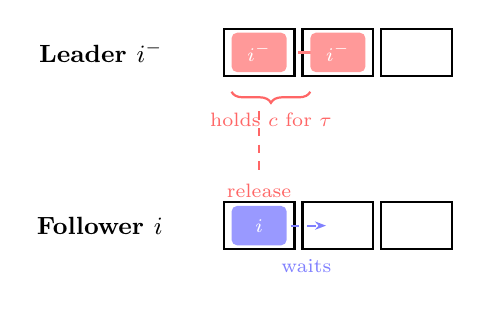
\begin{tikzpicture}[
    cell/.style={draw, thick, minimum width=0.9cm, minimum height=0.6cm, font=\scriptsize},
]
% Top: Leader i^-
\node[font=\small\bfseries, anchor=east] at (-1.6, 2.8) {Leader $i^-$};
\node[cell] at (-0.5, 2.8) {};
\node[cell] at (0.5, 2.8) {};
\node[cell] at (1.5, 2.8) {};
% Leader in cell c
\fill[red!40, rounded corners=2pt] (-0.85,2.55) rectangle (-0.15,3.05);
\node[font=\scriptsize, white] at (-0.5,2.8) {$i^-$};
% Arrow: leader moves
\draw[-{Stealth[length=4pt]}, thick, red!50] (0.0,2.8) -- (0.35,2.8);
% Leader at c+1
\fill[red!40, rounded corners=2pt] (0.15,2.55) rectangle (0.85,3.05);
\node[font=\scriptsize, white] at (0.5,2.8) {$i^-$};

% Delayed release brace
\draw[decorate, decoration={brace, amplitude=4pt}, thick, red!60]
    (0.15,2.3) -- (-0.85,2.3)
    node[midway, below=4pt, font=\scriptsize, red!60] {holds $c$ for $\tau$};

% Release marker
\draw[thick, red!60, dashed] (-0.5, 2.05) -- (-0.5, 1.3);
\node[font=\scriptsize, red!60, anchor=north] at (-0.5, 1.25) {release};

% Bottom: Follower i
\node[font=\small\bfseries, anchor=east] at (-1.6, 0.6) {Follower $i$};
\node[cell] at (-0.5, 0.6) {};
\node[cell] at (0.5, 0.6) {};
\node[cell] at (1.5, 0.6) {};
\fill[blue!40, rounded corners=2pt] (-0.85,0.35) rectangle (-0.15,0.85);
\node[font=\scriptsize, white] at (-0.5,0.6) {$i$};
\draw[-{Stealth[length=4pt]}, thick, blue!50, dashed] (-0.1,0.6) -- (0.35,0.6);
\node[font=\scriptsize, blue!50, below] at (0.1, 0.3) {waits};
\end{tikzpicture}
\end{center}
\end{column}
\begin{column}{0.50\textwidth}
\vspace{0.3em}
\begin{block}{Emergent headway}
\vspace{0.2em}
\[
\boxed{h = \tau^{(i^-)} + \frac{\ell}{v}}
\]
\vspace{0.1em}
{\scriptsize Exactly Newell's $h = \tau + d/v$ with $d = \ell$}
\end{block}

\vspace{0.5em}
\begin{alertblock}{Key insight}
Headway is \textbf{not imposed by a rule}\\
but \textbf{emerges} from the resource protocol
\end{alertblock}

\vspace{0.5em}
{\small Passage-time form:}
\[
T(x, n) = T(x{+}d,\, n{-}1) + \tau
\]
\end{column}
\end{columns}
\end{frame}

% ----------------------------------------------------------
\begin{frame}{Event-Driven Driver Process}
\begin{columns}[T]
\begin{column}{0.48\textwidth}
\centering
{\small\bfseries Push-Based Reactive Architecture}

\vspace{0.5em}
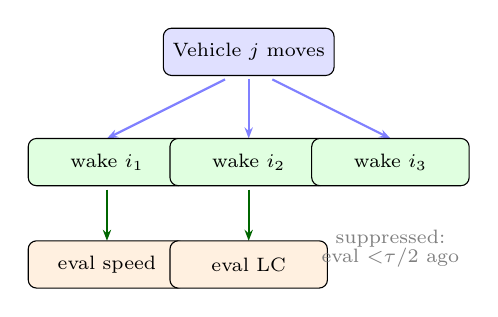
\begin{tikzpicture}[
    box/.style={draw, rounded corners=3pt, minimum width=2.0cm, minimum height=0.6cm,
                align=center, font=\scriptsize},
    arr/.style={-{Stealth[length=4pt]}, thick},
]
% Vehicle j moves — triggers cascade
\node[box, fill=blue!12] (jmove) at (0, 2.6) {Vehicle $j$ moves};
\draw[arr, blue!50] (-0.3, 2.25) -- (-1.8, 1.5);
\draw[arr, blue!50] (0, 2.25) -- (0, 1.5);
\draw[arr, blue!50] (0.3, 2.25) -- (1.8, 1.5);

% Neighbors woken
\node[box, fill=green!12] (w1) at (-1.8, 1.2) {wake $i_1$};
\node[box, fill=green!12] (w2) at (0, 1.2) {wake $i_2$};
\node[box, fill=green!12] (w3) at (1.8, 1.2) {wake $i_3$};

% Re-evaluate
\draw[arr, green!40!black] (-1.8, 0.85) -- (-1.8, 0.2);
\draw[arr, green!40!black] (0, 0.85) -- (0, 0.2);
\node[box, fill=orange!12] at (-1.8, -0.1) {eval speed};
\node[box, fill=orange!12] at (0, -0.1) {eval LC};
\node[font=\scriptsize, gray, align=center] at (1.8, 0.1) {suppressed:\\[-1pt] eval ${<}\tau/2$ ago};
\end{tikzpicture}
\end{column}
\begin{column}{0.48\textwidth}
\centering
{\small\bfseries Effort Follows Interactions}

\vspace{0.5em}
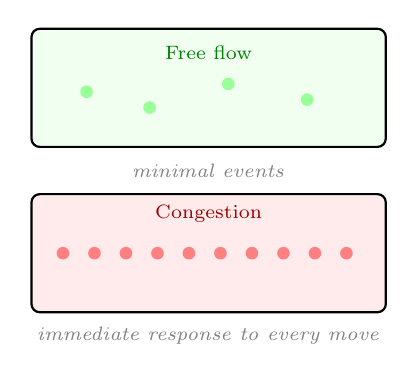
\begin{tikzpicture}
% Free flow region
\draw[thick, rounded corners=3pt, fill=green!6] (0,1.5) rectangle (4.5,3.0);
\node[font=\scriptsize, green!50!black] at (2.25, 2.7) {Free flow};
\foreach \x/\y in {0.7/2.2, 1.5/2.0, 2.5/2.3, 3.5/2.1} {
    \fill[green!40] (\x,\y) circle (0.08);
}
\node[font=\scriptsize, gray] at (2.25,1.2) {\textit{minimal events}};

% Congested region
\draw[thick, rounded corners=3pt, fill=red!8] (0,-0.6) rectangle (4.5,0.9);
\node[font=\scriptsize, red!60!black] at (2.25, 0.65) {Congestion};
\foreach \x in {0.4,0.8,1.2,1.6,2.0,2.4,2.8,3.2,3.6,4.0} {
    \fill[red!50] (\x,0.15) circle (0.08);
}
\node[font=\scriptsize, gray] at (2.25,-0.9) {\textit{immediate response to every move}};
\end{tikzpicture}
\end{column}
\end{columns}

\vspace{0.3em}
\centering
\fbox{\small Computational effort $\propto$ interacting vehicles, not total $N$}
\end{frame}

% ----------------------------------------------------------
\begin{frame}{Deterministic Lane-Change Models}
\begin{center}
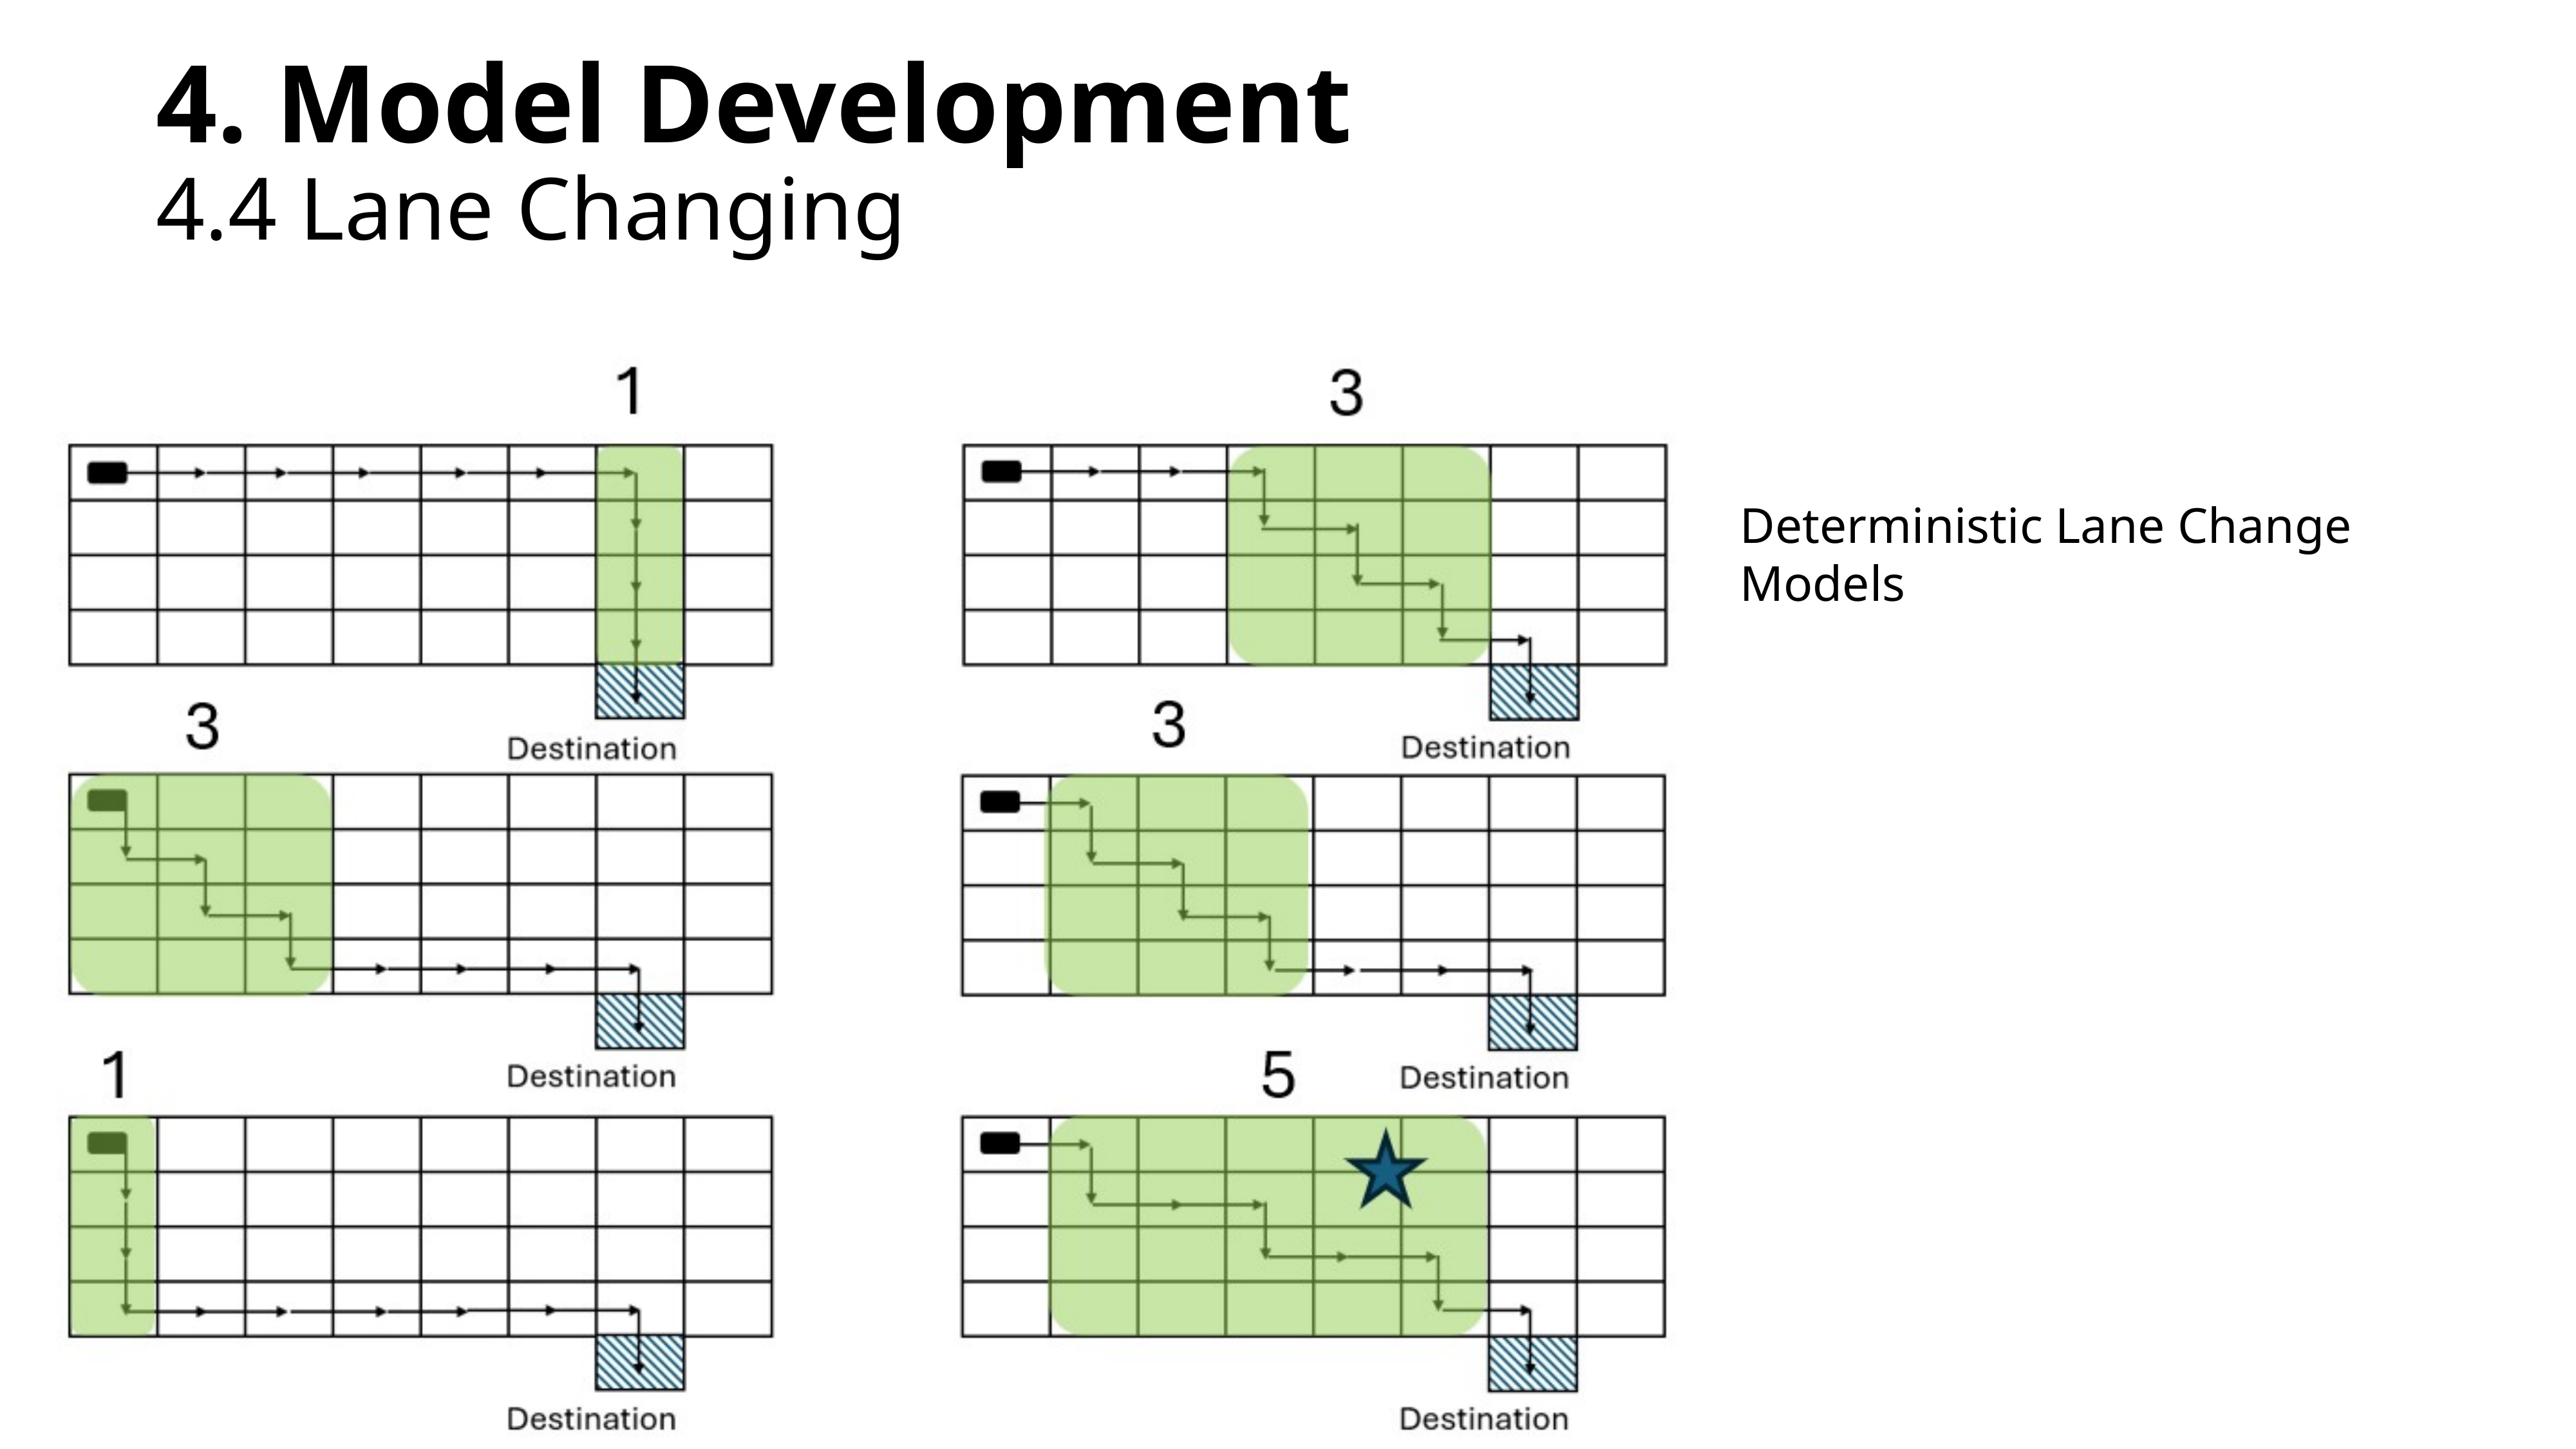
\includegraphics[width=0.88\textwidth,height=0.75\textheight,keepaspectratio]{diss_slide18-18.png}
\end{center}
\vspace{-0.5em}
{\small MLC path planning on a cell grid: vehicles navigate toward destinations via feasible lane-change sequences.}
\end{frame}

% ----------------------------------------------------------
\begin{frame}{Mandatory Lane Changing --- Logistic Functions}
\begin{columns}[T]
\begin{column}{0.40\textwidth}
\vspace{1em}
\textbf{Standard logistic function:}

\vspace{0.8em}
\[
f(x) = \frac{L}{1 + e^{-k(x - x_0)}}
\]

\vspace{1.5em}
{\small Standard form: $L=1,\; k=1,\; x_0=0$}

\vspace{1em}
{\small
\begin{itemize}
\item Output bounded in $[0, 1]$
\item S-shaped (sigmoid) curve
\item Smooth, differentiable
\item $k$ controls steepness
\item $x_0$ shifts midpoint
\end{itemize}
}
\end{column}
\begin{column}{0.58\textwidth}
\begin{center}
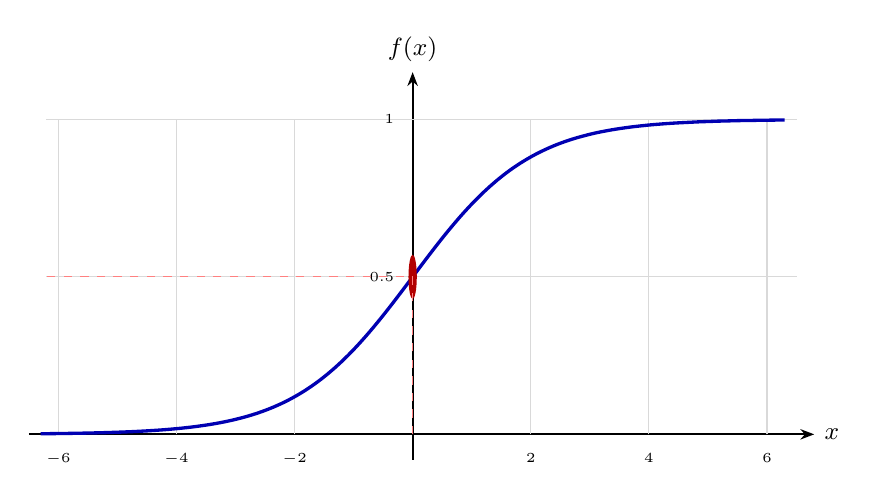
\begin{tikzpicture}[xscale=0.75, yscale=4.0]
% Axes
\draw[-{Stealth[length=5pt]}, thick] (-6.5,0) -- (6.8,0) node[right, font=\small] {$x$};
\draw[-{Stealth[length=5pt]}, thick] (0,-0.08) -- (0,1.15) node[above, font=\small] {$f(x)$};
% Grid lines
\foreach \x in {-6,-4,-2,2,4,6} {
    \draw[gray!30, thin] (\x,0) -- (\x,1.0);
    \node[font=\tiny, below] at (\x,-0.03) {$\x$};
}
\draw[gray!30, thin] (-6.2,0.5) -- (6.5,0.5);
\draw[gray!30, thin] (-6.2,1.0) -- (6.5,1.0);
\node[font=\tiny, left] at (-0.15,0.5) {0.5};
\node[font=\tiny, left] at (-0.15,1.0) {1};
% Sigmoid curve
\draw[blue!70!black, very thick, smooth, domain=-6.3:6.3, samples=100]
    plot (\x, {1/(1+exp(-\x))});
% Midpoint marker
\fill[red!70!black] (0,0.5) circle (2pt);
\draw[dashed, thin, red!50] (0,0) -- (0,0.5) -- (-6.2,0.5);
\end{tikzpicture}
\end{center}
\end{column}
\end{columns}
\end{frame}

% ----------------------------------------------------------
\begin{frame}[shrink=5]{Logistic Lane-Change Probability --- Justification}
\begin{center}
{\large $P_{\text{MLC}}(r, n) = \dfrac{1}{1 + e^{-k(r(n) - r)}}$}

\vspace{0.2em}
{\small Probability of mandatory lane change toward destination}
\end{center}

\vspace{0.3em}
\begin{columns}[T]
\begin{column}{0.48\textwidth}
\begin{block}{(i) Bounded Output}
{\small Logistic naturally produces probabilities in $[0,1]$, matching real-world decision-making constraints.}
\end{block}

\vspace{0.3em}
\begin{block}{(ii) S-shaped Curve}
{\small Sigmoid reflects natural progression of lane-changing urgency:}
\begin{itemize}
\item[\scriptsize$\bullet$] {\scriptsize Low probability far from destination}
\item[\scriptsize$\bullet$] {\scriptsize Rapid increase at critical distance}
\item[\scriptsize$\bullet$] {\scriptsize Saturation when very close}
\end{itemize}
\end{block}
\end{column}
\begin{column}{0.48\textwidth}
\begin{block}{(iii) Continuous \& Differentiable}
{\small Smooth transition reflects gradual change in driver behavior --- avoids unrealistic sudden jumps.}
\end{block}

\vspace{0.3em}
\begin{block}{(iv) Parametric Adaptability}
{\small Adjustable for:}
\begin{itemize}
\item[\scriptsize$\bullet$] {\scriptsize Different road configurations}
\item[\scriptsize$\bullet$] {\scriptsize Different driver populations}
\item[\scriptsize$\bullet$] {\scriptsize Scalable with number of lanes}
\end{itemize}
\end{block}
\end{column}
\end{columns}
\end{frame}

% ----------------------------------------------------------
\begin{frame}[shrink=15]{Lane-Change Models}
\begin{columns}[T]
\begin{column}{0.50\textwidth}
\begin{center}
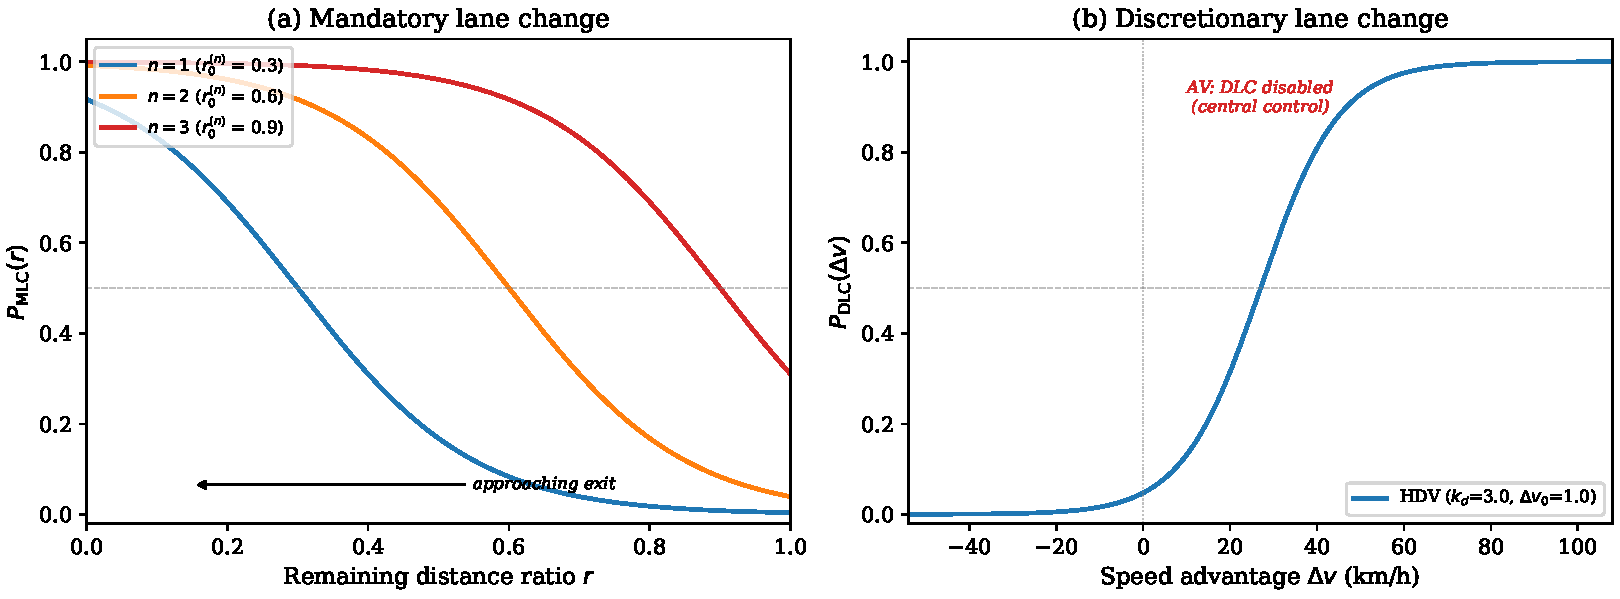
\includegraphics[width=\linewidth]{../figures/fig_lc_logistic.pdf}
\end{center}
\end{column}
\begin{column}{0.47\textwidth}
\vspace{0.5em}
\textbf{Mandatory LC} (approaching exit):
\[
P_{\text{MLC}}(r) = \frac{1}{1 + \exp\!\big({-}k(r_0 - r)\big)}
\]
{\scriptsize $r$ = fraction of trip remaining}

\vspace{0.5em}
\textbf{Discretionary LC} (speed gain):
\[
P_{\text{DLC}}(\Delta v) = \frac{1}{1 + \exp\!\big({-}k_d(\Delta v - \Delta v_0)\big)}
\]

\vspace{0.5em}
\textbf{Safety:} closing-speed gaps
{\scriptsize
\[
g_{\text{front}}^{\text{req}} = d + (g^{\max}_f - d) \cdot \frac{\max(0, v - v_L)}{v_{\max}}
\]}

\vspace{0.3em}
\textbf{Blockage:} $n_{\text{LC}} \mathrel{+}= 2$ when blockage detected\\
{\scriptsize $\rightarrow$ earlier merging at higher speeds}
\end{column}
\end{columns}
\end{frame}

% ----------------------------------------------------------
\section{Comparison with Classical CA}
% ==========================================================

% ----------------------------------------------------------
\begin{frame}[shrink=15]{ODCA-DES vs.\ NaSch: Side by Side}
\begin{center}
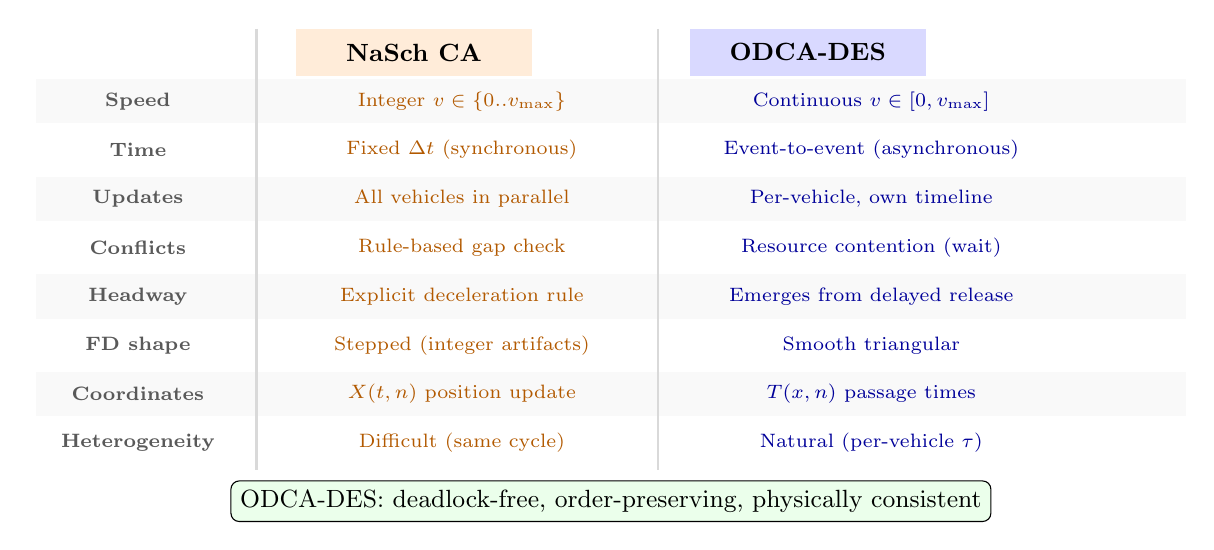
\begin{tikzpicture}[
    hdr/.style={font=\small\bfseries, minimum width=3cm, minimum height=0.6cm},
    cellL/.style={font=\scriptsize, minimum width=5.0cm, minimum height=0.55cm, align=left, anchor=west},
    cellR/.style={font=\scriptsize, minimum width=5.0cm, minimum height=0.55cm, align=left, anchor=west},
    dim/.style={font=\scriptsize\bfseries, minimum width=2.8cm, minimum height=0.55cm, align=right, anchor=east, text=gray!70!black},
]
% Headers
\node[hdr, fill=orange!15] at (-2.5, 3.2) {NaSch CA};
\node[hdr, fill=blue!15] at (2.5, 3.2) {ODCA-DES};

% Rows
% Row 1
\fill[gray!5] (-7.3,2.30) rectangle (7.3,2.86);
\node[dim] at (-4.6, 2.58) {Speed};
\node[cellL, text=orange!70!black] at (-4.4, 2.58) {Integer $v \in \{0..v_{\max}\}$};
\node[cellR, text=blue!60!black] at (0.8, 2.58) {Continuous $v \in [0, v_{\max}]$};
% Row 2
\node[dim] at (-4.6, 1.96) {Time};
\node[cellL, text=orange!70!black] at (-4.4, 1.96) {Fixed $\Delta t$ (synchronous)};
\node[cellR, text=blue!60!black] at (0.8, 1.96) {Event-to-event (asynchronous)};
% Row 3
\fill[gray!5] (-7.3,1.06) rectangle (7.3,1.62);
\node[dim] at (-4.6, 1.34) {Updates};
\node[cellL, text=orange!70!black] at (-4.4, 1.34) {All vehicles in parallel};
\node[cellR, text=blue!60!black] at (0.8, 1.34) {Per-vehicle, own timeline};
% Row 4
\node[dim] at (-4.6, 0.72) {Conflicts};
\node[cellL, text=orange!70!black] at (-4.4, 0.72) {Rule-based gap check};
\node[cellR, text=blue!60!black] at (0.8, 0.72) {Resource contention (wait)};
% Row 5
\fill[gray!5] (-7.3,-0.18) rectangle (7.3,0.38);
\node[dim] at (-4.6, 0.10) {Headway};
\node[cellL, text=orange!70!black] at (-4.4, 0.10) {Explicit deceleration rule};
\node[cellR, text=blue!60!black] at (0.8, 0.10) {Emerges from delayed release};
% Row 6
\node[dim] at (-4.6, -0.52) {FD shape};
\node[cellL, text=orange!70!black] at (-4.4, -0.52) {Stepped (integer artifacts)};
\node[cellR, text=blue!60!black] at (0.8, -0.52) {Smooth triangular};
% Row 7
\fill[gray!5] (-7.3,-1.42) rectangle (7.3,-0.86);
\node[dim] at (-4.6, -1.14) {Coordinates};
\node[cellL, text=orange!70!black] at (-4.4, -1.14) {$X(t,n)$ position update};
\node[cellR, text=blue!60!black] at (0.8, -1.14) {$T(x,n)$ passage times};
% Row 8
\node[dim] at (-4.6, -1.76) {Heterogeneity};
\node[cellL, text=orange!70!black] at (-4.4, -1.76) {Difficult (same cycle)};
\node[cellR, text=blue!60!black] at (0.8, -1.76) {Natural (per-vehicle $\tau$)};

% Vertical separator
\draw[thick, gray!30] (0.6, 3.5) -- (0.6, -2.1);
\draw[thick, gray!30] (-4.5, 3.5) -- (-4.5, -2.1);

% Bottom highlight
\node[draw, rounded corners=3pt, fill=green!8, font=\small, align=center] at (0, -2.5)
    {ODCA-DES: deadlock-free, order-preserving, physically consistent};
\end{tikzpicture}
\end{center}
\end{frame}

% ----------------------------------------------------------
\begin{frame}{Worked Example: Resource Contention in Action}
{\small Three vehicles: $A$@cell\,8 ($v{=}2$), $B$@cell\,5 ($v{=}3$), $C$@cell\,1 ($v{=}3$). $\tau = 1$\,s.}

\vspace{0.3em}
\begin{columns}[T]
\begin{column}{0.48\textwidth}
\centering
{\small\bfseries\color{orange!70!black} NaSch (synchronous)}

\vspace{0.3em}
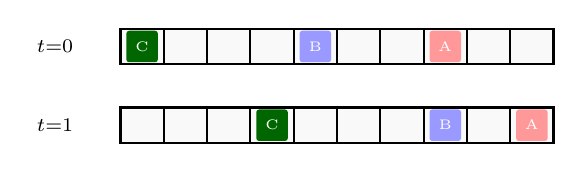
\begin{tikzpicture}[
    cell/.style={draw, thick, minimum width=0.55cm, minimum height=0.45cm, font=\tiny},
]
% t=0: cells 1-10
\node[font=\scriptsize, anchor=east] at (-0.2, 1.2) {$t{=}0$};
\foreach \x in {1,...,10} {
    \node[cell, fill=gray!5] at (\x*0.55, 1.2) {};
}
\fill[green!40!black, rounded corners=1pt] (1*0.55-0.2,1.0) rectangle (1*0.55+0.2,1.4);
\node[font=\tiny, white] at (1*0.55, 1.2) {C};
\fill[blue!40, rounded corners=1pt] (5*0.55-0.2,1.0) rectangle (5*0.55+0.2,1.4);
\node[font=\tiny, white] at (5*0.55, 1.2) {B};
\fill[red!40, rounded corners=1pt] (8*0.55-0.2,1.0) rectangle (8*0.55+0.2,1.4);
\node[font=\tiny, white] at (8*0.55, 1.2) {A};

% t=1
\node[font=\scriptsize, anchor=east] at (-0.2, 0.2) {$t{=}1$};
\foreach \x in {1,...,10} {
    \node[cell, fill=gray!5] at (\x*0.55, 0.2) {};
}
\fill[green!40!black, rounded corners=1pt] (4*0.55-0.2,0.0) rectangle (4*0.55+0.2,0.4);
\node[font=\tiny, white] at (4*0.55, 0.2) {C};
\fill[blue!40, rounded corners=1pt] (8*0.55-0.2,0.0) rectangle (8*0.55+0.2,0.4);
\node[font=\tiny, white] at (8*0.55, 0.2) {B};
\fill[red!40, rounded corners=1pt] (10*0.55-0.2,0.0) rectangle (10*0.55+0.2,0.4);
\node[font=\tiny, white] at (10*0.55, 0.2) {A};
\end{tikzpicture}

\vspace{0.2em}
{\scriptsize $B$ reaches cell 8 as $A$ departs ---\\simultaneous update allows this!}
\end{column}
\begin{column}{0.50\textwidth}
\centering
{\small\bfseries\color{blue!60!black} ODCA-DES (asynchronous)}

\vspace{0.3em}
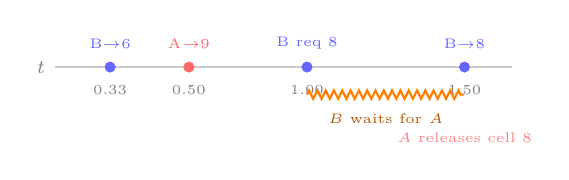
\begin{tikzpicture}
% Timeline
\draw[thick, gray!40] (0, 2.0) -- (5.8, 2.0);
\node[font=\scriptsize, gray, anchor=east] at (0, 2.0) {$t$};

% Events — timestamps above, labels below to avoid overlap
\fill[blue!60] (0.7, 2.0) circle (0.07);
\node[font=\tiny, blue!60, above=3pt] at (0.7, 2.0) {B$\to$6};
\node[font=\tiny, gray, below=3pt] at (0.7, 2.0) {0.33};

\fill[red!60] (1.7, 2.0) circle (0.07);
\node[font=\tiny, red!60, above=3pt] at (1.7, 2.0) {A$\to$9};
\node[font=\tiny, gray, below=3pt] at (1.7, 2.0) {0.50};

\fill[blue!60] (3.2, 2.0) circle (0.07);
\node[font=\tiny, blue!60, above=3pt] at (3.2, 2.0) {B req 8};
\node[font=\tiny, gray, below=3pt] at (3.2, 2.0) {1.00};

\fill[blue!60] (5.2, 2.0) circle (0.07);
\node[font=\tiny, blue!60, above=3pt] at (5.2, 2.0) {B$\to$8};
\node[font=\tiny, gray, below=3pt] at (5.2, 2.0) {1.50};

% Wait zigzag between B req 8 and B acq 8
\draw[thick, orange, decorate, decoration={zigzag, amplitude=1.5pt, segment length=3pt}]
    (3.2, 1.65) -- (5.2, 1.65);
\node[font=\tiny, orange!70!black] at (4.2, 1.35) {$B$ waits for $A$};

% Release marker centered under B->8
\node[font=\tiny, red!50] at (5.2, 1.1) {$A$ releases cell 8};
\end{tikzpicture}

\vspace{0.2em}
{\scriptsize Headway $= 1.5 - 0.5 = 1.0$\,s $= \tau$\\
(emerges from protocol)}
\end{column}
\end{columns}

\vspace{0.5em}
\centering
\fbox{\small NaSch: gap-check rules \qquad ODCA-DES: resource contention \emph{inherently} prevents collisions}
\end{frame}

% ==========================================================
\section{Computational Experiments}
% ==========================================================

% ----------------------------------------------------------
\begin{frame}{Experimental Setup}
\begin{columns}[T]
\begin{column}{0.45\textwidth}
\textbf{Key parameters:}

\vspace{0.3em}
\begin{center}
{\scriptsize
\begin{tabular}{@{}llcc@{}}
\toprule
& & HDV & AV \\
\midrule
$\tau$ & reaction & 1.5\,s & 0.5\,s \\
$v_{\max}$ & speed & 140\,km/h & 140\,km/h \\
$p$ & slowdown & 0.15 & 0.0 \\
$\Delta v_0$ & DLC thresh & 1.0 & 0.4 \\
\bottomrule
\end{tabular}
}
\end{center}

\vspace{0.3em}
\textbf{HDV heterogeneity:}\\
{\scriptsize $\tau_i \!\sim\! \text{LogN}(1.5, 0.3)$, \;
$\delta_i \!\sim\! \text{LogN}(1.0, 0.2)$, \;
$p_i \!\sim\! \mathcal{N}(0.15, 0.05)$}
\end{column}
\begin{column}{0.52\textwidth}
\textbf{Scenarios:}

\vspace{0.3em}
\begin{center}
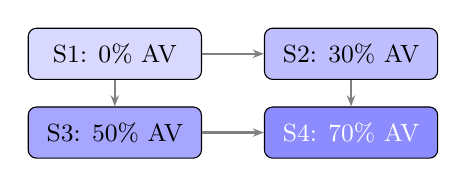
\begin{tikzpicture}[
    sbox/.style={draw, rounded corners=3pt, minimum width=2.2cm, minimum height=0.65cm,
                 font=\small, align=center},
]
\node[sbox, fill=blue!15] (s1) at (0,0) {S1: 0\% AV};
\node[sbox, fill=blue!25] (s2) at (3,0) {S2: 30\% AV};
\node[sbox, fill=blue!35] (s3) at (0,-1.0) {S3: 50\% AV};
\node[sbox, fill=blue!45, text=white] (s4) at (3,-1.0) {S4: 70\% AV};

\draw[-{Stealth[length=4pt]}, thick, gray] (s1) -- (s2);
\draw[-{Stealth[length=4pt]}, thick, gray] (s2) -- (s4);
\draw[-{Stealth[length=4pt]}, thick, gray] (s1) -- (s3);
\draw[-{Stealth[length=4pt]}, thick, gray] (s3) -- (s4);
\end{tikzpicture}
\end{center}

\vspace{0.3em}
{\small 4-lane, 6\,km freeway\\
10 replications per scenario\\
$T_{\text{sim}} = 3600$\,s}
\end{column}
\end{columns}
\end{frame}

% ----------------------------------------------------------
\begin{frame}{FD Validation: ODCA-DES vs.\ NaSch}
\begin{columns}[T]
\begin{column}{0.72\textwidth}
\begin{center}
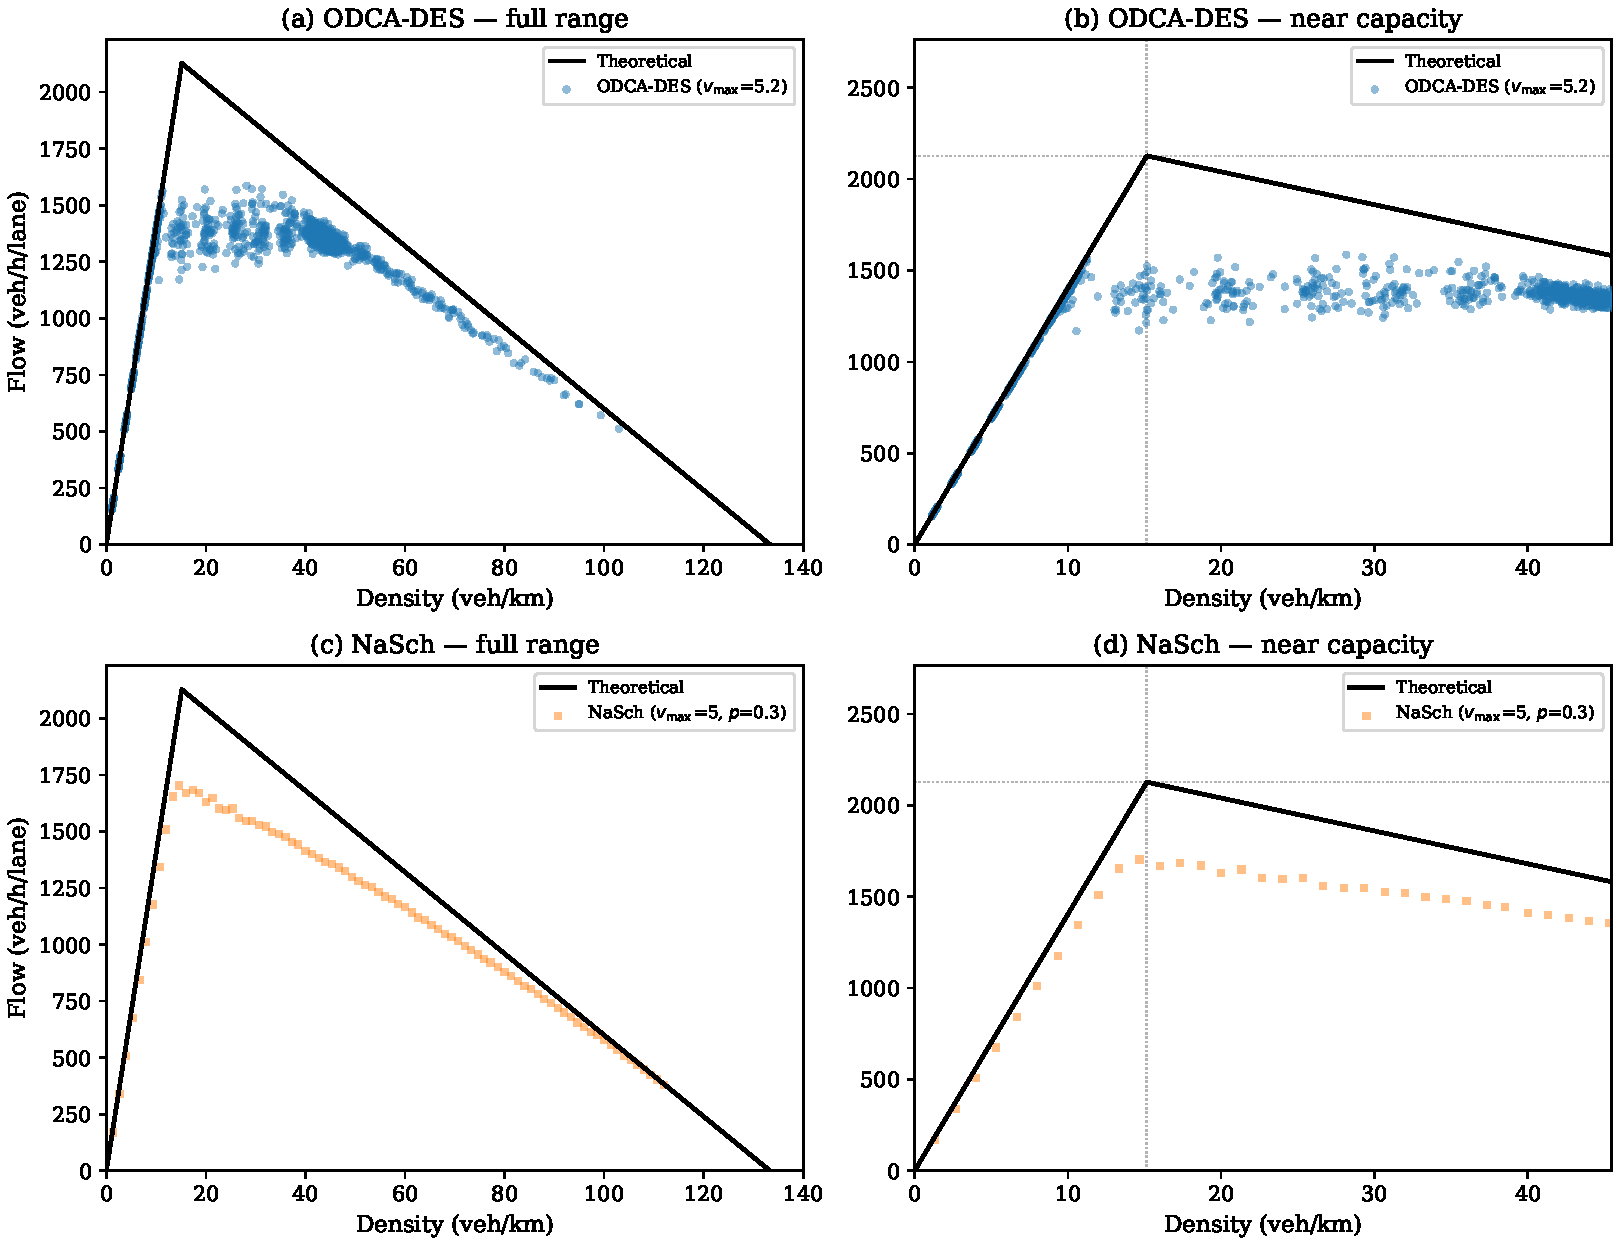
\includegraphics[width=\textwidth,height=0.78\textheight,keepaspectratio]{../figures/fig_fd_theoretical.pdf}
\end{center}
\end{column}
\begin{column}{0.26\textwidth}
\vspace{0.5em}
{\scriptsize\bfseries Setup:}\\[3pt]
{\scriptsize
Ring road, 400 cells\\
$\ell = 7.5$\,m (3\,km)\\
HDV only, homogeneous\\[4pt]
$\tau = 1.5$\,s, $d = 1$ cell\\
$v_{\max} = 5.2$\,cells/s\\
$p = 0.15$ (slowdown)\\[4pt]
Density init: 25 levels\\
Edie's FD, 20\,s windows\\
Meas.\ region: cells 100--300\\[6pt]
}
{\scriptsize\bfseries NaSch equiv.:}\\[3pt]
{\scriptsize
$v_{\max} = 5$ cells/step\\
$\Delta t = 1$\,s\\
Same $p$, density range
}

\vspace{0.8em}
{\scriptsize
\textbf{Top:} ODCA-DES --- smooth\\
\textbf{Bottom:} NaSch --- staircase
}
\end{column}
\end{columns}
\end{frame}

% ----------------------------------------------------------
\begin{frame}{Multi-Lane Fundamental Diagram}
\begin{center}
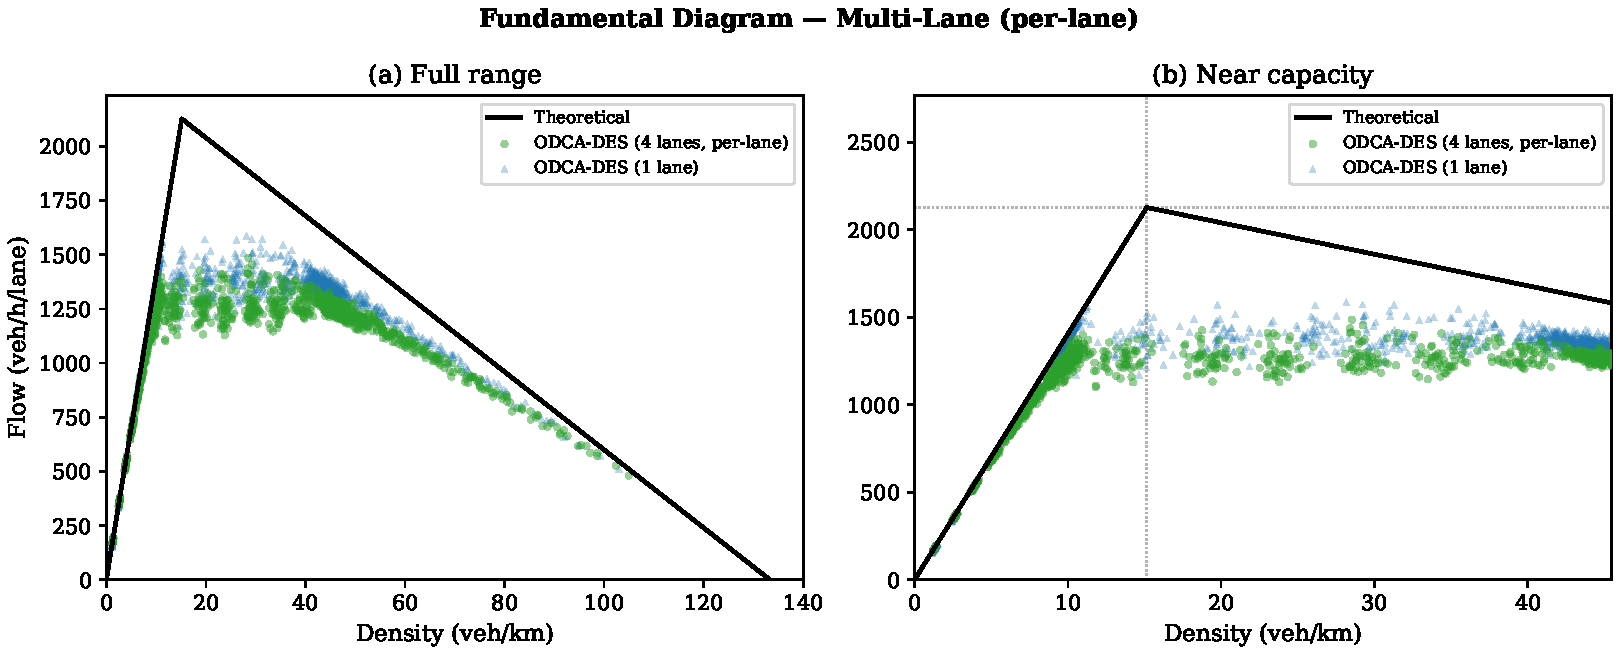
\includegraphics[width=0.88\textwidth,height=0.82\textheight,keepaspectratio]{../figures/fig_fd_multi_lane.pdf}
\end{center}
\end{frame}

% ----------------------------------------------------------
\begin{frame}{Mixed AV/HDV Traffic: Capacity Benefit}
\begin{columns}[T]
\begin{column}{0.52\textwidth}
\begin{center}
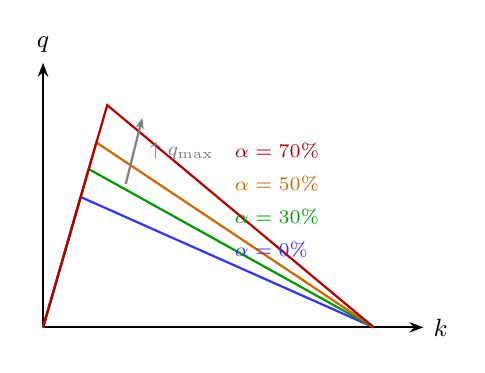
\begin{tikzpicture}[xscale=4.2, yscale=2.8]
% Axes
\draw[-{Stealth[length=5pt]}, thick] (0,0) -- (1.15,0) node[right, font=\small] {$k$};
\draw[-{Stealth[length=5pt]}, thick] (0,0) -- (0,1.2) node[above, font=\small] {$q$};

% FDs for different alpha values
\draw[blue!80, thick] (0,0) -- (0.114,0.591) -- (1.0,0);
\draw[green!60!black, thick] (0,0) -- (0.138,0.718) -- (1.0,0);
\draw[orange!80!black, thick] (0,0) -- (0.161,0.839) -- (1.0,0);
\draw[red!70!black, thick] (0,0) -- (0.194,1.008) -- (1.0,0);

% Legend — placed inside congested region to avoid axis overlap
\node[font=\scriptsize, blue!80, anchor=west] at (0.55,0.35) {$\alpha = 0\%$};
\node[font=\scriptsize, green!60!black, anchor=west] at (0.55,0.50) {$\alpha = 30\%$};
\node[font=\scriptsize, orange!80!black, anchor=west] at (0.55,0.65) {$\alpha = 50\%$};
\node[font=\scriptsize, red!70!black, anchor=west] at (0.55,0.80) {$\alpha = 70\%$};

% Capacity arrow
\draw[-{Stealth[length=4pt]}, thick, gray] (0.25,0.65) -- (0.30,0.95)
    node[midway, right=2pt, font=\scriptsize, gray] {$\uparrow q_{\max}$};
\end{tikzpicture}
\end{center}
\end{column}
\begin{column}{0.45\textwidth}
\vspace{0.3em}
Headway depends on \emph{leader's} $\tau$:

\vspace{0.3em}
\[
\boxed{q_{\max}(\alpha) = \frac{v_f}{v_f\bar{\tau}(\alpha) + \ell}}
\]

{\scriptsize where $\bar{\tau} = \alpha \tau_{\text{AV}} + (1{-}\alpha)\tau_{\text{HDV}}$}

\vspace{0.5em}
\begin{center}
{\small
\begin{tabular}{@{}cccc@{}}
\toprule
$\alpha$ & $\bar{\tau}$ & $q_{\max}$ & Gain \\
\midrule
0\% & 1.50\,s & 2127 & --- \\
30\% & 1.20\,s & 2586 & +22\% \\
50\% & 1.00\,s & 3019 & +42\% \\
70\% & 0.80\,s & 3628 & +71\% \\
\bottomrule
\end{tabular}
}
\end{center}

\vspace{0.3em}
{\small Driven entirely by $\tau_{\text{AV}} = 0.5$\,s vs.\ $\tau_{\text{HDV}} = 1.5$\,s}
\end{column}
\end{columns}
\end{frame}

% ==========================================================
\begin{frame}{Time-Space Diagrams: Free Flow vs.\ Congestion}
\begin{center}
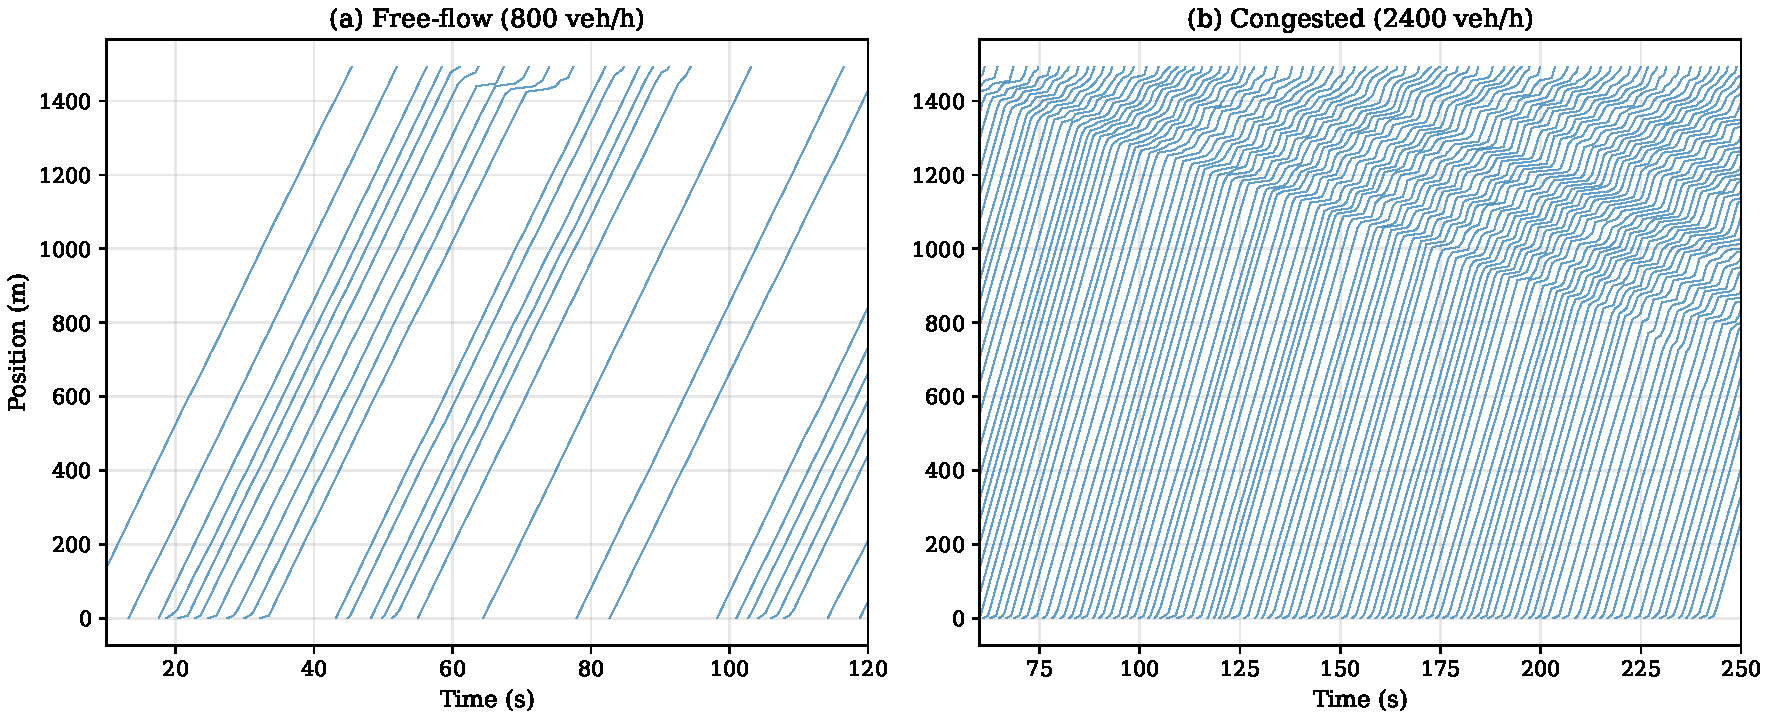
\includegraphics[width=0.88\textwidth,height=0.72\textheight,keepaspectratio]{../figures/fig_tsd_combined.pdf}
\end{center}
\vspace{-0.3em}
{\small
\textbf{(a)} Free flow: parallel trajectories at $v_f \approx 140$\,km/h. \quad
\textbf{(b)} Congested: backward waves at $w \approx 18$\,km/h.
}
\end{frame}

% ----------------------------------------------------------
\begin{frame}{Delay Concentration: Travel Speed vs.\ Running Speed}
\begin{center}
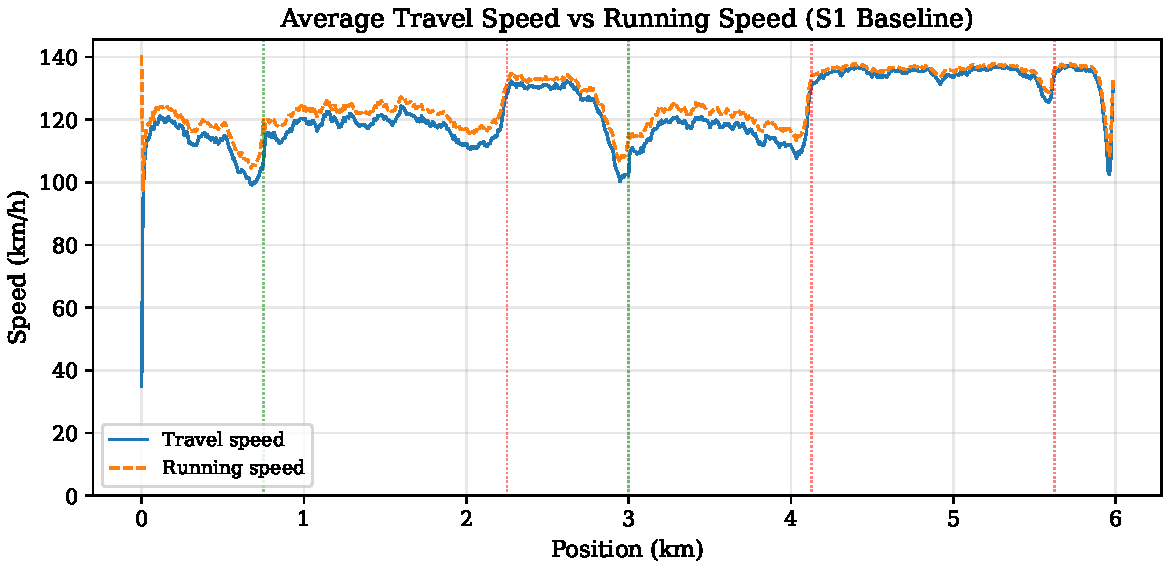
\includegraphics[width=0.88\textwidth,height=0.72\textheight,keepaspectratio]{../figures/fig_speed_profile.pdf}
\end{center}
\vspace{-0.3em}
\centering
{\small Gap = delay from lane-changing friction upstream of off-ramps}
\end{frame}

% ----------------------------------------------------------
\begin{frame}[shrink=12]{Mixed Traffic Results}
\begin{columns}[T]
\begin{column}{0.48\textwidth}
\begin{center}
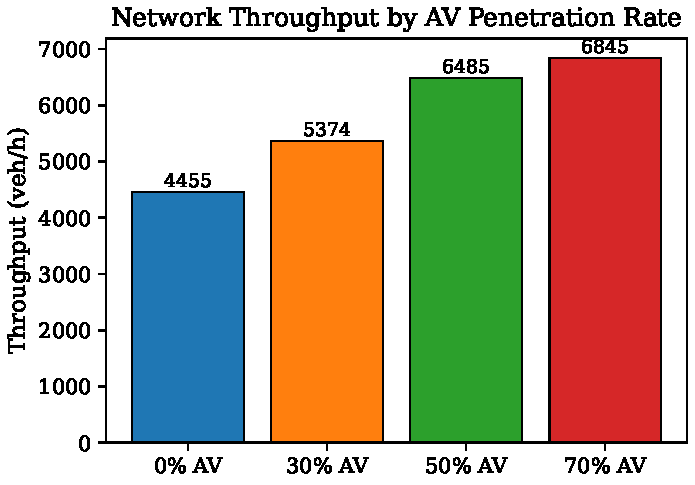
\includegraphics[width=\linewidth]{../figures/fig_throughput_bar.pdf}
\end{center}
\end{column}
\begin{column}{0.48\textwidth}
\begin{center}
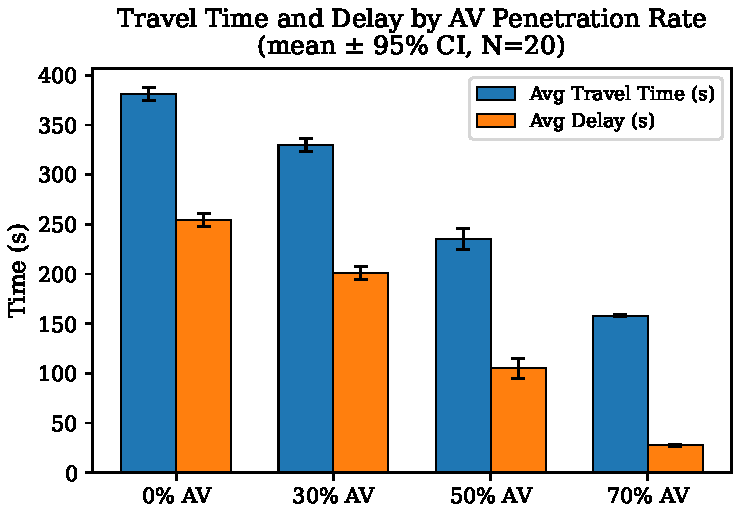
\includegraphics[width=\linewidth]{../figures/fig_travel_time.pdf}
\end{center}
\end{column}
\end{columns}

\vspace{0.5em}
\begin{center}
{\small
\begin{tabular}{@{}lcccc@{}}
\toprule
& S1 (0\%) & S2 (30\%) & S3 (50\%) & S4 (70\%) \\
\midrule
Throughput (veh/h) & 4419 & 4905 & 5515 & \textbf{6531} {\scriptsize (+48\%)} \\
Avg.\ delay (s) & 266 & 229 & 206 & \textbf{111} {\scriptsize ($-$58\%)} \\
\bottomrule
\end{tabular}
}
\end{center}
\end{frame}

% ==========================================================
\section{Incident Scenario}
% ==========================================================

% ----------------------------------------------------------
\begin{frame}[shrink=12]{Dynamic Congestion: Lane-Closure Incident}
\begin{center}
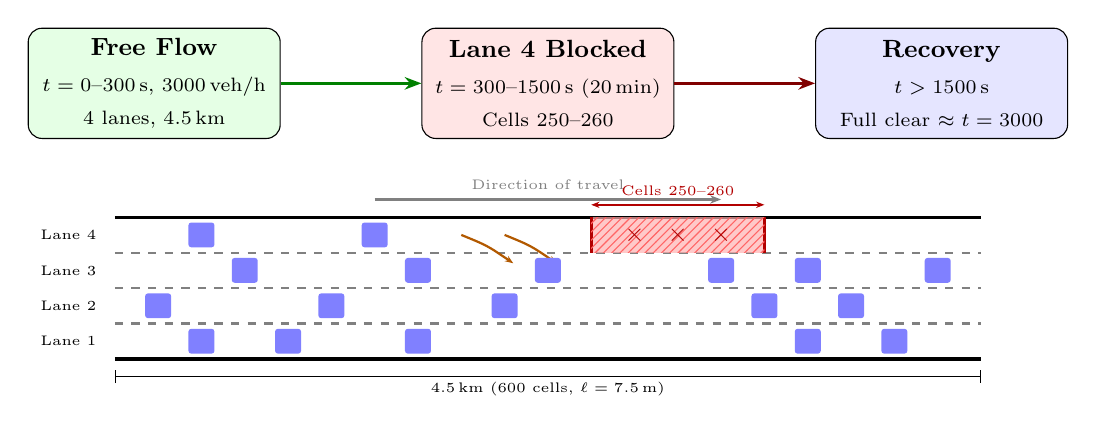
\begin{tikzpicture}[
    phase/.style={draw, rounded corners=5pt, minimum width=3.2cm, minimum height=1.4cm,
                  align=center, font=\small},
    arr/.style={-{Stealth[length=6pt]}, very thick},
]
% Phase 1: Free flow
\node[phase, fill=green!10] (p1) at (-5, 1.5) {
    \textbf{Free Flow}\\[2pt]
    {\scriptsize $t = 0$--$300$\,s, 3000\,veh/h}\\[1pt]
    {\scriptsize 4 lanes, 4.5\,km}
};

% Phase 2: Incident
\node[phase, fill=red!10] (p2) at (0, 1.5) {
    \textbf{Lane 4 Blocked}\\[2pt]
    {\scriptsize $t = 300$--$1500$\,s (20\,min)}\\[1pt]
    {\scriptsize Cells 250--260}
};

% Phase 3: Recovery
\node[phase, fill=blue!10] (p3) at (5, 1.5) {
    \textbf{Recovery}\\[2pt]
    {\scriptsize $t > 1500$\,s}\\[1pt]
    {\scriptsize Full clear $\approx t=3000$}
};

\draw[arr, green!50!black] (p1) -- (p2);
\draw[arr, red!50!black] (p2) -- (p3);

% --- Freeway lane-closure diagram ---
% 4-lane freeway segment
\begin{scope}[shift={(0,-2.0)}, x=1.1cm, y=0.45cm]
% Lane boundaries
\draw[very thick] (-5,0) -- (5,0);
\draw[thick, dashed, gray] (-5,1) -- (5,1);
\draw[thick, dashed, gray] (-5,2) -- (5,2);
\draw[thick, dashed, gray] (-5,3) -- (5,3);
\draw[very thick] (-5,4) -- (5,4);

% Lane labels
\node[font=\tiny, anchor=east] at (-5.1,0.5) {Lane 1};
\node[font=\tiny, anchor=east] at (-5.1,1.5) {Lane 2};
\node[font=\tiny, anchor=east] at (-5.1,2.5) {Lane 3};
\node[font=\tiny, anchor=east] at (-5.1,3.5) {Lane 4};

% Direction arrow
\draw[-{Stealth[length=4pt]}, thick, gray] (-2,4.5) -- (2,4.5);
\node[font=\tiny, gray, above] at (0,4.5) {Direction of travel};

% Blocked region on Lane 4 (cells 250-260)
\fill[red!30, opacity=0.7] (0.5,3) rectangle (2.5,4);
\draw[red!70!black, very thick] (0.5,3) -- (0.5,4);
\draw[red!70!black, very thick] (2.5,3) -- (2.5,4);
\fill[pattern=north east lines, pattern color=red!60] (0.5,3) rectangle (2.5,4);

% X marks in blocked area
\node[font=\small, red!70!black] at (1.0,3.5) {$\times$};
\node[font=\small, red!70!black] at (1.5,3.5) {$\times$};
\node[font=\small, red!70!black] at (2.0,3.5) {$\times$};

% Label for blocked region
\draw[{Stealth[length=3pt]}-{Stealth[length=3pt]}, thick, red!70!black] (0.5,4.35) -- (2.5,4.35);
\node[font=\tiny, red!70!black, above] at (1.5,4.35) {Cells 250--260};

% Vehicles merging (arrows showing LC from lane 4 to lane 3)
\draw[-{Stealth[length=3pt]}, thick, orange!70!black] (-0.5,3.5) .. controls (-0.2,3.2) .. (0.1,2.7);
\draw[-{Stealth[length=3pt]}, thick, orange!70!black] (-1.0,3.5) .. controls (-0.7,3.2) .. (-0.4,2.7);

% Vehicles in lanes (small blue rectangles)
\foreach \x in {-4.0,-3.0,-1.5,3.0,4.0} {
    \fill[blue!50, rounded corners=1pt] (\x-0.15,0.15) rectangle (\x+0.15,0.85);
}
\foreach \x in {-4.5,-2.5,-0.5,2.5,3.5} {
    \fill[blue!50, rounded corners=1pt] (\x-0.15,1.15) rectangle (\x+0.15,1.85);
}
\foreach \x in {-3.5,-1.5,0.0,2.0,3.0,4.5} {
    \fill[blue!50, rounded corners=1pt] (\x-0.15,2.15) rectangle (\x+0.15,2.85);
}
\foreach \x in {-4.0,-2.0} {
    \fill[blue!50, rounded corners=1pt] (\x-0.15,3.15) rectangle (\x+0.15,3.85);
}

% Distance label
\draw[|-|, thin] (-5,-0.5) -- (5,-0.5);
\node[font=\tiny] at (0,-0.85) {4.5\,km (600 cells, $\ell = 7.5$\,m)};
\end{scope}
\end{tikzpicture}
\end{center}
\end{frame}

% ----------------------------------------------------------
\begin{frame}{Incident: Time-Space Trajectories}
\begin{center}
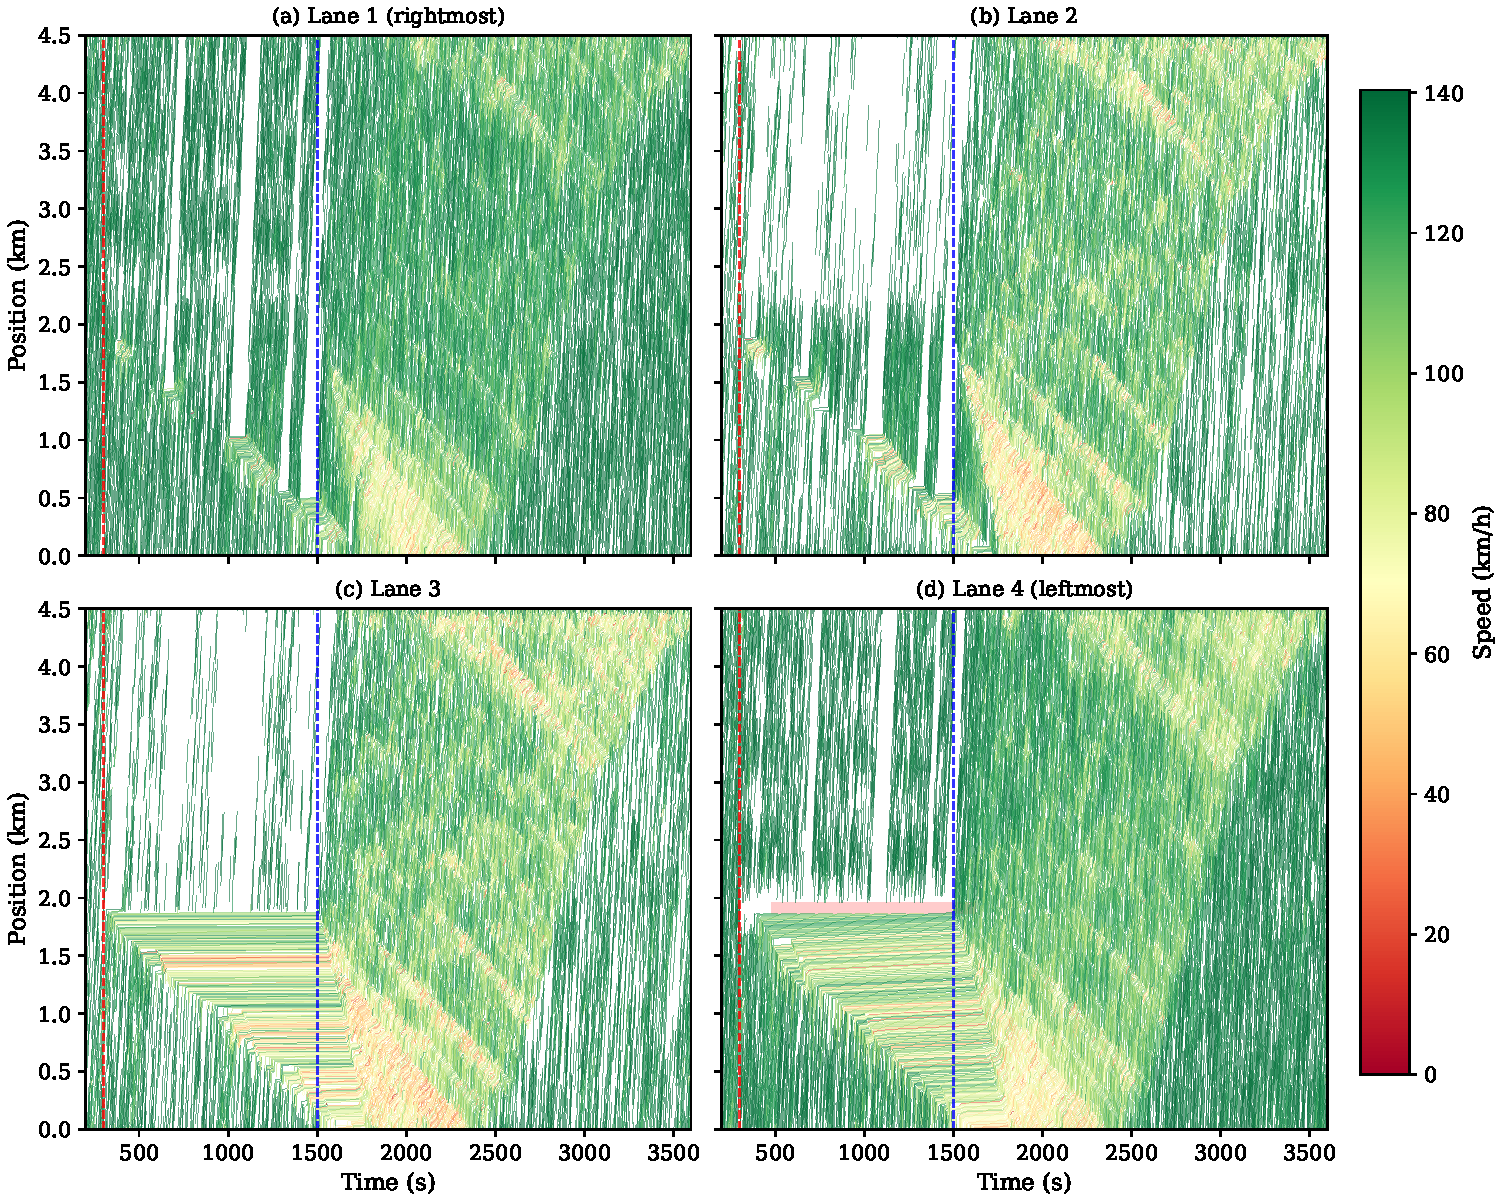
\includegraphics[width=0.95\textwidth,height=0.78\textheight,keepaspectratio]{../figures/fig_incident_trajectories.pdf}
\end{center}
\vspace{-0.5em}
{\small Left: uniform baseline. \quad Right: queue buildup, spillback, recovery after clearance.}
\end{frame}

% ----------------------------------------------------------
\begin{frame}{Incident: Density Heatmaps}
\begin{center}
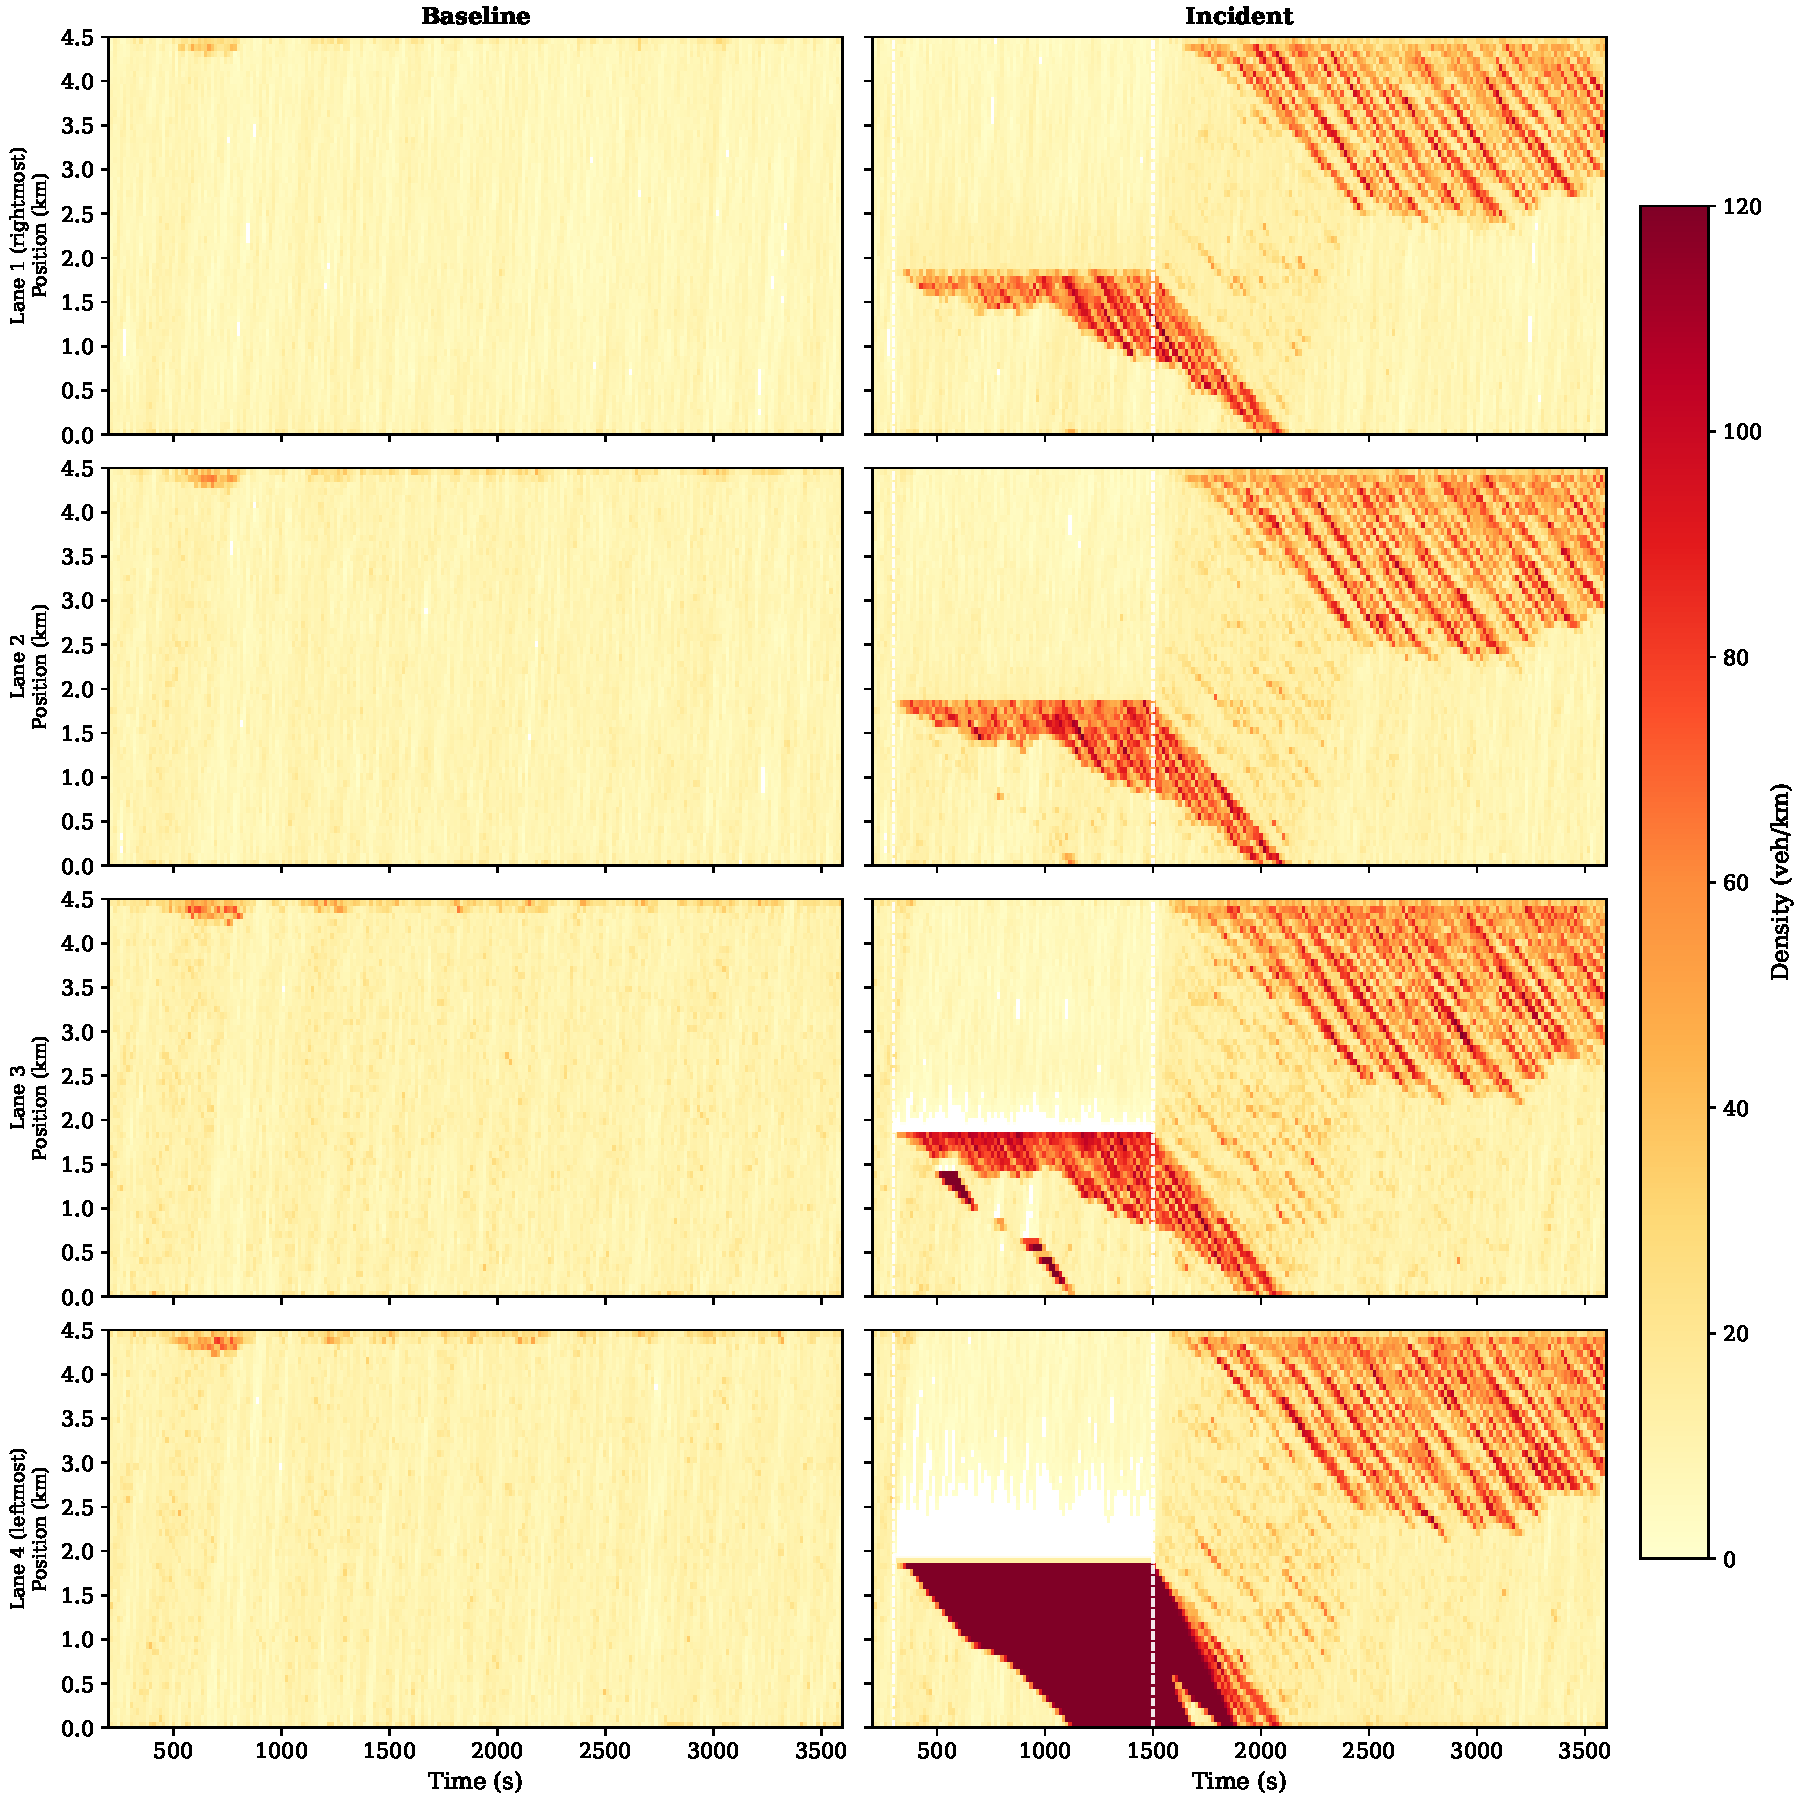
\includegraphics[width=0.95\textwidth,height=0.78\textheight,keepaspectratio]{../figures/fig_incident_heatmap.pdf}
\end{center}
\vspace{-0.5em}
{\small Backward waves as diagonal bands --- kinematic wave behavior from microscopic mechanics.}
\end{frame}

% ==========================================================
\section{Computational Performance}
% ==========================================================

% ----------------------------------------------------------
\begin{frame}[shrink=12]{Event-Driven Efficiency}
\begin{columns}[T]
\begin{column}{0.50\textwidth}
\begin{center}
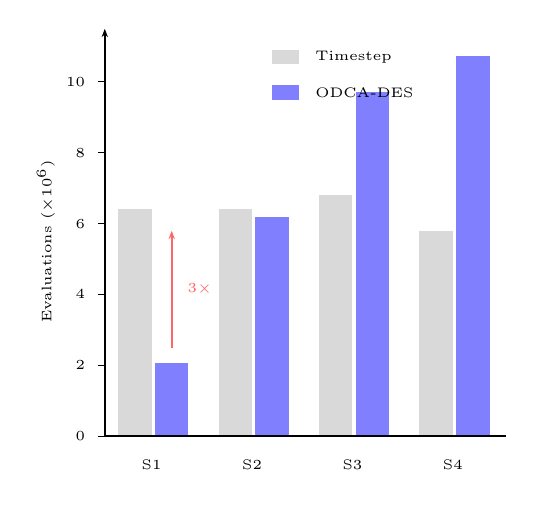
\begin{tikzpicture}[yscale=0.45, xscale=0.85]
% Bar chart: CF evals vs timestep updates

% Timestep baseline (gray bars)
\foreach \x/\val/\lbl in {0.5/6.4/S1, 2.0/6.4/S2, 3.5/6.8/S3, 5.0/5.8/S4} {
    \fill[gray!30] (\x, 0) rectangle (\x+0.5, \val);
    \node[font=\tiny, below] at (\x+0.5, -0.4) {\lbl};
}

% ODCA-DES CF evals (blue bars)
\foreach \x/\val in {0.5/2.08, 2.0/6.18, 3.5/9.71, 5.0/10.73} {
    \fill[blue!50] (\x+0.55, 0) rectangle (\x+1.05, \val);
}

% Y axis
\draw[-{Stealth[length=3pt]}, thick] (0.3,0) -- (0.3,11.5);
\foreach \y in {0,2,4,6,8,10} {
    \draw[thin] (0.2,\y) -- (0.3,\y);
    \node[font=\tiny, anchor=east] at (0.15,\y) {\y};
}
\node[font=\tiny, rotate=90, anchor=south] at (-0.3, 5.5) {Evaluations ($\times 10^6$)};

% X axis
\draw[thick] (0.3,0) -- (6.3,0);

% Legend
\fill[gray!30] (2.8, 10.5) rectangle (3.2, 10.9);
\node[font=\tiny, anchor=west] at (3.3, 10.7) {Timestep};
\fill[blue!50] (2.8, 9.5) rectangle (3.2, 9.9);
\node[font=\tiny, anchor=west] at (3.3, 9.7) {ODCA-DES};

% Annotation
\draw[-{Stealth[length=3pt]}, thick, red!60] (1.3, 2.5) -- (1.3, 5.8)
    node[midway, right=2pt, font=\tiny, red!60] {$3\times$};
\end{tikzpicture}
\end{center}
\end{column}
\begin{column}{0.47\textwidth}
\vspace{1em}
\begin{center}
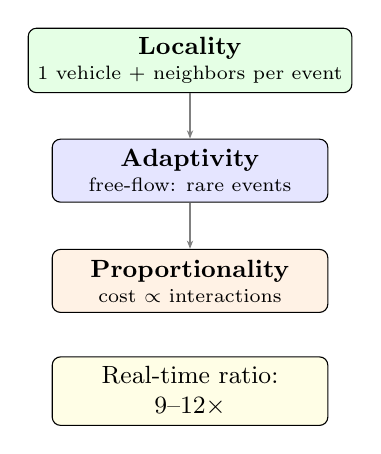
\begin{tikzpicture}[
    box/.style={draw, rounded corners=3pt, minimum width=3.5cm, minimum height=0.8cm,
                font=\small, align=center},
]
\node[box, fill=green!10] (loc) at (0, 2.0) {\textbf{Locality}\\[-2pt] {\scriptsize 1 vehicle + neighbors per event}};
\node[box, fill=blue!10] (adp) at (0, 0.6) {\textbf{Adaptivity}\\[-2pt] {\scriptsize free-flow: rare events}};
\node[box, fill=orange!10] (prop) at (0, -0.8) {\textbf{Proportionality}\\[-2pt] {\scriptsize cost $\propto$ interactions}};

\draw[-{Stealth[length=3pt]}, thick, gray] (loc) -- (adp);
\draw[-{Stealth[length=3pt]}, thick, gray] (adp) -- (prop);

\node[draw, rounded corners=3pt, fill=yellow!10, font=\small, align=center,
      minimum width=3.5cm] at (0, -2.2) {Real-time ratio:\\$9$--$12\times$};
\end{tikzpicture}
\end{center}
\end{column}
\end{columns}
\end{frame}

% ==========================================================
\section{Conclusions}
% ==========================================================

% ----------------------------------------------------------
\begin{frame}[shrink=12]{Key Contributions}
\begin{center}
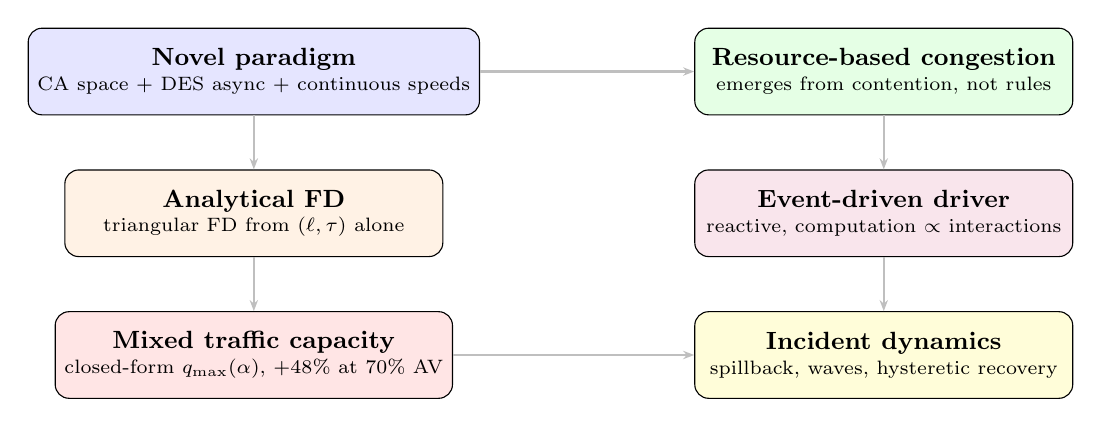
\begin{tikzpicture}[
    cbox/.style={draw, rounded corners=5pt, minimum width=4.8cm, minimum height=1.1cm,
                 align=center, font=\small},
    arr/.style={-{Stealth[length=4pt]}, thick, gray!50},
]
% Top row
\node[cbox, fill=blue!10] (c1) at (-4, 2.0) {\textbf{Novel paradigm}\\[-2pt] {\scriptsize CA space + DES async + continuous speeds}};
\node[cbox, fill=green!10] (c2) at (4, 2.0) {\textbf{Resource-based congestion}\\[-2pt] {\scriptsize emerges from contention, not rules}};

% Middle row
\node[cbox, fill=orange!10] (c3) at (-4, 0.2) {\textbf{Analytical FD}\\[-2pt] {\scriptsize triangular FD from $(\ell, \tau)$ alone}};
\node[cbox, fill=purple!10] (c4) at (4, 0.2) {\textbf{Event-driven driver}\\[-2pt] {\scriptsize reactive, computation $\propto$ interactions}};

% Bottom row
\node[cbox, fill=red!10] (c5) at (-4, -1.6) {\textbf{Mixed traffic capacity}\\[-2pt] {\scriptsize closed-form $q_{\max}(\alpha)$, +48\% at 70\% AV}};
\node[cbox, fill=yellow!15] (c6) at (4, -1.6) {\textbf{Incident dynamics}\\[-2pt] {\scriptsize spillback, waves, hysteretic recovery}};

% Connecting arrows
\draw[arr] (c1) -- (c3);
\draw[arr] (c2) -- (c4);
\draw[arr] (c3) -- (c5);
\draw[arr] (c4) -- (c6);
\draw[arr] (c1) -- (c2);
\draw[arr] (c5) -- (c6);
\end{tikzpicture}
\end{center}
\end{frame}

% ----------------------------------------------------------
\begin{frame}{Limitations and Future Directions}
\begin{columns}[T]
\begin{column}{0.45\textwidth}
\begin{center}
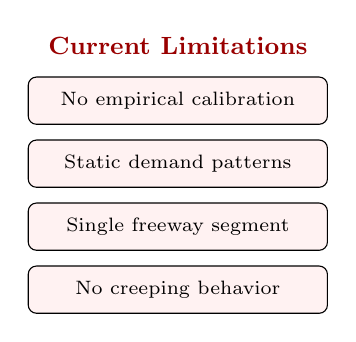
\begin{tikzpicture}[
    item/.style={draw, rounded corners=3pt, minimum width=3.8cm, minimum height=0.6cm,
                 font=\scriptsize, align=center, fill=red!5},
]
\node[font=\small\bfseries, red!60!black] at (0, 2.5) {Current Limitations};
\node[item] at (0, 1.8) {No empirical calibration};
\node[item] at (0, 1.0) {Static demand patterns};
\node[item] at (0, 0.2) {Single freeway segment};
\node[item] at (0, -0.6) {No creeping behavior};
\end{tikzpicture}
\end{center}
\end{column}
\begin{column}{0.52\textwidth}
\begin{center}
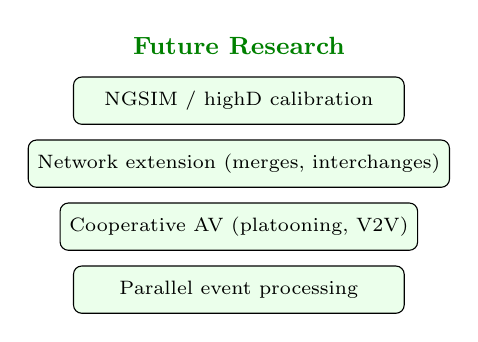
\begin{tikzpicture}[
    item/.style={draw, rounded corners=3pt, minimum width=4.2cm, minimum height=0.6cm,
                 font=\scriptsize, align=center, fill=green!8},
]
\node[font=\small\bfseries, green!50!black] at (0, 2.5) {Future Research};
\node[item] at (0, 1.8) {NGSIM / highD calibration};
\node[item] at (0, 1.0) {Network extension (merges, interchanges)};
\node[item] at (0, 0.2) {Cooperative AV (platooning, V2V)};
\node[item] at (0, -0.6) {Parallel event processing};
\end{tikzpicture}
\end{center}
\end{column}
\end{columns}
\end{frame}

% ----------------------------------------------------------
{
\setbeamercolor{background canvas}{bg=white}
\setbeamercolor{block body}{bg=white, fg=black}
\setbeamercolor{normal text}{fg=black}
\begin{frame}[plain]{References}
\frametitle{References}
{\scriptsize\color{black}
\begin{enumerate}
\item[{[1]}] G.\,F.\ Newell, ``A simplified theory of kinematic waves in highway traffic, Part I--III,'' \textit{Transp.\ Res.\ B}, 27(4), 281--313, 1993.
\item[{[2]}] G.\,F.\ Newell, ``A simplified car-following theory: a lower order model,'' \textit{Transp.\ Res.\ B}, 36(3), 195--205, 2002.
\item[{[3]}] K.\ Nagel, M.\ Schreckenberg, ``A cellular automaton model for freeway traffic,'' \textit{J.\ de Physique I}, 2(12), 2221--2229, 1992.
\item[{[4]}] M.\ Rickert et al., ``Two lane traffic simulations using cellular automata,'' \textit{Physica A}, 231(4), 534--550, 1996.
\item[{[5]}] W.\ Knospe et al., ``Towards a realistic microscopic description of highway traffic,'' \textit{J.\ Phys.\ A}, 33(48), L477, 2000.
\item[{[6]}] M.\,J.\ Lighthill, G.\,B.\ Whitham, ``On kinematic waves II,'' \textit{Proc.\ Roy.\ Soc.\ A}, 229, 317--345, 1955.
\item[{[7]}] P.\,I.\ Richards, ``Shock waves on the highway,'' \textit{Oper.\ Res.}, 4(1), 42--51, 1956.
\item[{[8]}] L.\,C.\ Edie, ``Discussion of traffic stream measurements and definitions,'' \textit{Proc.\ 2nd Int.\ Symp.\ Theory of Traffic Flow}, 139--154, 1963.
\end{enumerate}
}
\end{frame}
}

% ----------------------------------------------------------
\begin{frame}
\centering
\vspace{0.8cm}

% Little AV cars driving across
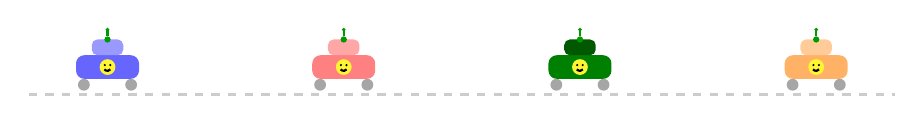
\begin{tikzpicture}
% Car 1 (left)
\begin{scope}[shift={(-4.5,0)}, scale=0.5]
  \fill[blue!60, rounded corners=3pt] (-0.8,-0.3) rectangle (0.8,0.3);
  \fill[blue!40, rounded corners=2pt] (-0.4,0.3) rectangle (0.4,0.7);
  \fill[gray!70] (-0.6,-0.45) circle (0.15);
  \fill[gray!70] (0.6,-0.45) circle (0.15);
  % Sensor on top
  \fill[green!60!black] (0,0.7) circle (0.08);
  \draw[green!60!black, thick] (0,0.78) -- (0,0.95);
  \fill[green!60!black] (0,0.95) circle (0.05);
  % Smiley face on side
  \fill[yellow!80] (0,0.0) circle (0.2);
  \fill[black] (-0.07,0.05) circle (0.03);
  \fill[black] (0.07,0.05) circle (0.03);
  \draw[black, thick] (-0.08,-0.06) arc[start angle=220, end angle=320, radius=0.1];
\end{scope}

% Car 2 (center-left)
\begin{scope}[shift={(-1.5,0)}, scale=0.5]
  \fill[red!50, rounded corners=3pt] (-0.8,-0.3) rectangle (0.8,0.3);
  \fill[red!35, rounded corners=2pt] (-0.4,0.3) rectangle (0.4,0.7);
  \fill[gray!70] (-0.6,-0.45) circle (0.15);
  \fill[gray!70] (0.6,-0.45) circle (0.15);
  \fill[green!60!black] (0,0.7) circle (0.08);
  \draw[green!60!black, thick] (0,0.78) -- (0,0.95);
  \fill[green!60!black] (0,0.95) circle (0.05);
  \fill[yellow!80] (0,0.0) circle (0.2);
  \fill[black] (-0.07,0.05) circle (0.03);
  \fill[black] (0.07,0.05) circle (0.03);
  \draw[black, thick] (-0.08,-0.06) arc[start angle=220, end angle=320, radius=0.1];
\end{scope}

% Car 3 (center-right)
\begin{scope}[shift={(1.5,0)}, scale=0.5]
  \fill[green!50!black, rounded corners=3pt] (-0.8,-0.3) rectangle (0.8,0.3);
  \fill[green!35!black, rounded corners=2pt] (-0.4,0.3) rectangle (0.4,0.7);
  \fill[gray!70] (-0.6,-0.45) circle (0.15);
  \fill[gray!70] (0.6,-0.45) circle (0.15);
  \fill[green!60!black] (0,0.7) circle (0.08);
  \draw[green!60!black, thick] (0,0.78) -- (0,0.95);
  \fill[green!60!black] (0,0.95) circle (0.05);
  \fill[yellow!80] (0,0.0) circle (0.2);
  \fill[black] (-0.07,0.05) circle (0.03);
  \fill[black] (0.07,0.05) circle (0.03);
  \draw[black, thick] (-0.08,-0.06) arc[start angle=220, end angle=320, radius=0.1];
\end{scope}

% Car 4 (right)
\begin{scope}[shift={(4.5,0)}, scale=0.5]
  \fill[orange!60, rounded corners=3pt] (-0.8,-0.3) rectangle (0.8,0.3);
  \fill[orange!40, rounded corners=2pt] (-0.4,0.3) rectangle (0.4,0.7);
  \fill[gray!70] (-0.6,-0.45) circle (0.15);
  \fill[gray!70] (0.6,-0.45) circle (0.15);
  \fill[green!60!black] (0,0.7) circle (0.08);
  \draw[green!60!black, thick] (0,0.78) -- (0,0.95);
  \fill[green!60!black] (0,0.95) circle (0.05);
  \fill[yellow!80] (0,0.0) circle (0.2);
  \fill[black] (-0.07,0.05) circle (0.03);
  \fill[black] (0.07,0.05) circle (0.03);
  \draw[black, thick] (-0.08,-0.06) arc[start angle=220, end angle=320, radius=0.1];
\end{scope}

% Road line
\draw[gray!40, thick, dashed] (-5.5,-0.35) -- (5.5,-0.35);
\end{tikzpicture}

\vspace{1em}
{\Large Thank you!}

\vspace{1em}
{\large Questions?}

\vspace{1.5em}
{\normalsize Kerem Demirtas}\\
\texttt{kdemirta@asu.edu}\\
\vspace{0.5em}
School of Computing and Augmented Intelligence\\
Arizona State University
\end{frame}

\end{document}
